% Options for packages loaded elsewhere
\PassOptionsToPackage{unicode}{hyperref}
\PassOptionsToPackage{hyphens}{url}
\PassOptionsToPackage{dvipsnames,svgnames,x11names}{xcolor}
%
\documentclass[
  letterpaper,
  DIV=11,
  numbers=noendperiod]{scrartcl}

\usepackage{amsmath,amssymb}
\usepackage{iftex}
\ifPDFTeX
  \usepackage[T1]{fontenc}
  \usepackage[utf8]{inputenc}
  \usepackage{textcomp} % provide euro and other symbols
\else % if luatex or xetex
  \usepackage{unicode-math}
  \defaultfontfeatures{Scale=MatchLowercase}
  \defaultfontfeatures[\rmfamily]{Ligatures=TeX,Scale=1}
\fi
\usepackage{lmodern}
\ifPDFTeX\else  
    % xetex/luatex font selection
\fi
% Use upquote if available, for straight quotes in verbatim environments
\IfFileExists{upquote.sty}{\usepackage{upquote}}{}
\IfFileExists{microtype.sty}{% use microtype if available
  \usepackage[]{microtype}
  \UseMicrotypeSet[protrusion]{basicmath} % disable protrusion for tt fonts
}{}
\makeatletter
\@ifundefined{KOMAClassName}{% if non-KOMA class
  \IfFileExists{parskip.sty}{%
    \usepackage{parskip}
  }{% else
    \setlength{\parindent}{0pt}
    \setlength{\parskip}{6pt plus 2pt minus 1pt}}
}{% if KOMA class
  \KOMAoptions{parskip=half}}
\makeatother
\usepackage{xcolor}
\setlength{\emergencystretch}{3em} % prevent overfull lines
\setcounter{secnumdepth}{5}
% Make \paragraph and \subparagraph free-standing
\ifx\paragraph\undefined\else
  \let\oldparagraph\paragraph
  \renewcommand{\paragraph}[1]{\oldparagraph{#1}\mbox{}}
\fi
\ifx\subparagraph\undefined\else
  \let\oldsubparagraph\subparagraph
  \renewcommand{\subparagraph}[1]{\oldsubparagraph{#1}\mbox{}}
\fi


\providecommand{\tightlist}{%
  \setlength{\itemsep}{0pt}\setlength{\parskip}{0pt}}\usepackage{longtable,booktabs,array}
\usepackage{calc} % for calculating minipage widths
% Correct order of tables after \paragraph or \subparagraph
\usepackage{etoolbox}
\makeatletter
\patchcmd\longtable{\par}{\if@noskipsec\mbox{}\fi\par}{}{}
\makeatother
% Allow footnotes in longtable head/foot
\IfFileExists{footnotehyper.sty}{\usepackage{footnotehyper}}{\usepackage{footnote}}
\makesavenoteenv{longtable}
\usepackage{graphicx}
\makeatletter
\def\maxwidth{\ifdim\Gin@nat@width>\linewidth\linewidth\else\Gin@nat@width\fi}
\def\maxheight{\ifdim\Gin@nat@height>\textheight\textheight\else\Gin@nat@height\fi}
\makeatother
% Scale images if necessary, so that they will not overflow the page
% margins by default, and it is still possible to overwrite the defaults
% using explicit options in \includegraphics[width, height, ...]{}
\setkeys{Gin}{width=\maxwidth,height=\maxheight,keepaspectratio}
% Set default figure placement to htbp
\makeatletter
\def\fps@figure{htbp}
\makeatother
\newlength{\cslhangindent}
\setlength{\cslhangindent}{1.5em}
\newlength{\csllabelwidth}
\setlength{\csllabelwidth}{3em}
\newlength{\cslentryspacingunit} % times entry-spacing
\setlength{\cslentryspacingunit}{\parskip}
\newenvironment{CSLReferences}[2] % #1 hanging-ident, #2 entry spacing
 {% don't indent paragraphs
  \setlength{\parindent}{0pt}
  % turn on hanging indent if param 1 is 1
  \ifodd #1
  \let\oldpar\par
  \def\par{\hangindent=\cslhangindent\oldpar}
  \fi
  % set entry spacing
  \setlength{\parskip}{#2\cslentryspacingunit}
 }%
 {}
\usepackage{calc}
\newcommand{\CSLBlock}[1]{#1\hfill\break}
\newcommand{\CSLLeftMargin}[1]{\parbox[t]{\csllabelwidth}{#1}}
\newcommand{\CSLRightInline}[1]{\parbox[t]{\linewidth - \csllabelwidth}{#1}\break}
\newcommand{\CSLIndent}[1]{\hspace{\cslhangindent}#1}

\usepackage{booktabs}
\usepackage{longtable}
\usepackage{array}
\usepackage{multirow}
\usepackage{wrapfig}
\usepackage{float}
\usepackage{colortbl}
\usepackage{pdflscape}
\usepackage{tabu}
\usepackage{threeparttable}
\usepackage{threeparttablex}
\usepackage[normalem]{ulem}
\usepackage{makecell}
\usepackage{xcolor}
\usepackage{cancel}
\addtokomafont{disposition}{\rmfamily}
\KOMAoption{captions}{tableheading}
\makeatletter
\makeatother
\makeatletter
\makeatother
\makeatletter
\@ifpackageloaded{caption}{}{\usepackage{caption}}
\AtBeginDocument{%
\ifdefined\contentsname
  \renewcommand*\contentsname{Table of contents}
\else
  \newcommand\contentsname{Table of contents}
\fi
\ifdefined\listfigurename
  \renewcommand*\listfigurename{List of Figures}
\else
  \newcommand\listfigurename{List of Figures}
\fi
\ifdefined\listtablename
  \renewcommand*\listtablename{List of Tables}
\else
  \newcommand\listtablename{List of Tables}
\fi
\ifdefined\figurename
  \renewcommand*\figurename{Figure}
\else
  \newcommand\figurename{Figure}
\fi
\ifdefined\tablename
  \renewcommand*\tablename{Table}
\else
  \newcommand\tablename{Table}
\fi
}
\@ifpackageloaded{float}{}{\usepackage{float}}
\floatstyle{ruled}
\@ifundefined{c@chapter}{\newfloat{codelisting}{h}{lop}}{\newfloat{codelisting}{h}{lop}[chapter]}
\floatname{codelisting}{Listing}
\newcommand*\listoflistings{\listof{codelisting}{List of Listings}}
\usepackage{amsthm}
\theoremstyle{plain}
\newtheorem{proposition}{Proposition}[section]
\theoremstyle{plain}
\newtheorem{lemma}{Lemma}[section]
\theoremstyle{remark}
\AtBeginDocument{\renewcommand*{\proofname}{Proof}}
\newtheorem*{remark}{Remark}
\newtheorem*{solution}{Solution}
\makeatother
\makeatletter
\@ifpackageloaded{caption}{}{\usepackage{caption}}
\@ifpackageloaded{subcaption}{}{\usepackage{subcaption}}
\makeatother
\makeatletter
\@ifpackageloaded{tcolorbox}{}{\usepackage[skins,breakable]{tcolorbox}}
\makeatother
\makeatletter
\@ifundefined{shadecolor}{\definecolor{shadecolor}{rgb}{.97, .97, .97}}
\makeatother
\makeatletter
\makeatother
\makeatletter
\makeatother
\ifLuaTeX
  \usepackage{selnolig}  % disable illegal ligatures
\fi
\IfFileExists{bookmark.sty}{\usepackage{bookmark}}{\usepackage{hyperref}}
\IfFileExists{xurl.sty}{\usepackage{xurl}}{} % add URL line breaks if available
\urlstyle{same} % disable monospaced font for URLs
\hypersetup{
  pdftitle={The behavioral effects of index insurance in fisheries},
  pdfauthor={Nathaniel Grimes; Christopher Costello; Andrew J. Plantinga},
  pdfkeywords={Index Insurance, Moral Hazard, Fisheries, Conservation},
  colorlinks=true,
  linkcolor={blue},
  filecolor={Maroon},
  citecolor={Blue},
  urlcolor={Blue},
  pdfcreator={LaTeX via pandoc}}

\title{The behavioral effects of index insurance in fisheries}
\usepackage{etoolbox}
\makeatletter
\providecommand{\subtitle}[1]{% add subtitle to \maketitle
  \apptocmd{\@title}{\par {\large #1 \par}}{}{}
}
\makeatother
\subtitle{Working Paper Draft \emph{Not For Circulation}}
\author{Nathaniel Grimes \and Christopher Costello \and Andrew J.
Plantinga}
\date{2024-11-13}

\begin{document}
\maketitle
\begin{abstract}
Fisheries are vulnerable to environmental shocks that impact stock
health and fisher income. Index insurance is a promising financial tool
to protect fishers from environmental risk. However, insurance will
change fisher's behavior through moral hazards. We provide the first
theoretical application of index insurance on fisher's behavior change
to predict if index insurance will incentivize overfishing or
conservation of the stock. Using traditional fishery models will always
bias index insurance to incentivize overfishing, which in turn reduces
fish stocks. However, using models with more flexible input risk effects
shows index insurance will have varying effects on fishery conservation.
The direction of change depends on the risk characteristics of the
inputs. We find that index insurance will raise (lower) individual
fisher effort when effort is risk increasing (decreasing). In turn,
higher (lower) fishing effort reduces (increases) conservation of fish
stocks. The direction of harvest change becomes ambiguous when
accounting for interaction between multiple inputs. Simulating from
parameters estimated for four Norwegian fisheries shows index inusrance
could increase harvest as high as 15\% or decrease harvest by 6\%.
Before widespread adoption, careful consideration must be given to how
index insurance will incentivize or disincentivize overfishing.
\end{abstract}
\ifdefined\Shaded\renewenvironment{Shaded}{\begin{tcolorbox}[interior hidden, enhanced, sharp corners, frame hidden, boxrule=0pt, borderline west={3pt}{0pt}{shadecolor}, breakable]}{\end{tcolorbox}}\fi

\renewcommand*\contentsname{Table of contents}
{
\hypersetup{linkcolor=}
\setcounter{tocdepth}{3}
\tableofcontents
}
\hypertarget{introduction}{%
\section{Introduction}\label{introduction}}

Fishing is a vital economic engine to coastal communities and is the
primary source of protein for millions of people (Sumaila \emph{et al.}
2012; Teh and Sumaila 2013; FAO 2020). Supporting these communities
requires protection from enormous degrees of environmental risk.
Environmental fluctuations directly impact fishers of all scales from
large industrial vessels to small scale subsistence fishers.

Marine heatwaves provide a clear example of how environmental
variability impacts fishery biological and economic productivity. Marine
heatwaves increase animal thermal stress diminishing reproductive
ability (Barbeaux \emph{et al.} 2020), stunting growth (Pandori and
Sorte 2019), pushing species outside their usual habitats (Cavole
\emph{et al.} 2016), and may directly increase mortality (Smith \emph{et
al.} 2023). Expanding fish habitat ranges increase costs when moving
beyond the fishing grounds of established ports (Rogers \emph{et al.}
2019). The variability from marine heatwaves alone impacts 77\% of
species within economic exclusion zones and reduces maximum catch
potential by 6\% (Cheung \emph{et al.} 2021). Marine heatwaves are often
accompanied by harmful algal blooms and diseases leading to additional
fishery collapses (Oken \emph{et al.} 2021).

Weather can also impact fisher harvesting efficiency beyond influencing
the health of the underlying stock. Rolling seas and high wind speeds
make it more difficult to harvest (Alvarez \emph{et al.} 2006) in
addition to raising the danger to crew and vessel (Heck \emph{et al.}
2021). More intense storms threaten coastal infrastructure vital to
fishing communities (Sainsbury \emph{et al.} 2019). Fishers actively
avoid fishing in destructive weather at the expense of lost income
(Pfeiffer 2020).

Individual choices by fishers and fishery management mitigate
environmental risk. Fishers are highly sensitive to risk, especially
income risk, and demonstrate risk aversion despite working a seemingly
risky profession (Smith and Wilen 2005; Holland 2008; Sethi 2010).
Individual efforts to mitigate risk such as choosing consistent, known
fishing grounds over risking exploring unknown spots (Holland 2008) or
choosing to fish less after storms and hurricanes (Pfeiffer 2020;
Pfeiffer \emph{et al.} 2022) are likely to be incomplete and that
financial tools like insurance could further help fishers. However,
there is a lack of financial tools available to fishers to address
income risk as a result of environmental fluctuations (Sethi 2010;
Kasperski and Holland 2013). There is growing interest in developing new
financial tools to alleviate financial and income risk for coastal
communities (Wabnitz and Blasiak 2019; Sumaila \emph{et al.} 2020).

Insurance may be an ideal financial tool for risk management in
fisheries as it is scalable, protects against environmental shocks, and
smooths income for fishers (Watson \emph{et al.} 2023). Currently,
insurance in fisheries is primarily used to protect assets such as
vessel hulls or fishing gear (FAO 2022). Insurance coverage could be
expanded to include income variability originating from weather and
biological productivity shocks. An insurance product covering these
environmental risks could improve fisher welfare and promote community
resilience (Maltby \emph{et al.} 2023).

Policy makers have begun advocating for new fisheries insurance programs
modeled after agricultural crop insurance programs (Murkowski 2022).
Index insurance is one such product extolled by practitioners as a prime
candidate for fisheries productivity insurance (Watson \emph{et al.}
2023). Index insurance gained traction in agriculture as an effective
alternative to traditional crop insurance in developing countries
because it had lower administrative cost, minimized moral hazards, and
does not require claim verification (Collier \emph{et al.} 2009; Carter
\emph{et al.} 2017). Whereas indemnity crop insurance requires an
assessment of loss to an individual farm, index insurance uses an
independent measure as the basis for issuing payouts to all
policyholders. For example, a pilot program through the Caribbean Oceans
and Aqauculture Sustainability Facility (COAST) uses index insurance to
payout a set amount to fishers when indices of wave height, wind speed,
and storm surge indicate a hurricane (Sainsbury \emph{et al.} 2019).
Triggers are the index values that initiate a payout. Contract design
revolve around establishing suitable triggers to cover environmental
loss.

One crucial area that remains under studied is the potential influence
of insurance on fishers behavior. Moral hazards are decisions by insured
agents that they would not otherwise take if they were uninsured (Wu
\emph{et al.} 2020). Currently, the operational assumption of
practitioners appears to be that index insurance would completely avoid
any moral hazards in fisheries and intrinsically motivate greater
fishery sustainability {[}ORAA?{]}. Yet, there are two components to
insurance moral hazard: ``chasing the trigger'' and ``risk reduction''.
``Chasing the trigger'' is the directed behavior of policyholders to
increase the likelihood of a payout. For example, a fisher actively
choosing to fish less to receive an indemnified harvest insurance
payment. Index insurance completely eliminates this moral hazard through
the independent and uninfluenced index (fishers cannot affect sea
surface temperature). ``Risk reduction'' occurs through possessing an
insurance contract that protects policyholders from risk. Policyholders
may reoptimize their decisions once protected from risk. Index insurance
remains susceptible to this element of moral hazard that could manifest
in maladaptive behaviors. In fisheries, it could be choosing to fish
more when insurance covers losses. All preliminary analyses of fisheries
index insurance are missing rigorous assessment of this element of moral
hazards.

Previous studies in agriculture provide compelling evidence that
behavior change ought to be expected in fisheries. Index insurance
applied to grazing in pasture commons shows clear evidence of risk
reduction moral hazards (Müller \emph{et al.} 2011; Bulte and Haagsma
2021). Other studies from agriculture describe a more equivocal
relationship between insurance and environmental sustainability. The
impact of insurance on environmental sustainability depends on the
underlying risk reducing or increasing qualities of inputs used in
production (Ramaswami 1993; Mahul 2001; Mishra \emph{et al.} 2005). Risk
increasing inputs will always lead to increased input use with
insurance, while risk decreasing inputs will always lead to decreased
input use with insurance. Numerous agricultural studies confirm the
insurance incentivizes changes in inputs (Horowitz and Lichtenberg 1993;
Babcock and Hennessy 1996; Smith and Goodwin 1996; Goodwin \emph{et al.}
2004; Mishra \emph{et al.} 2005; Cai 2016; Deryugina and Konar 2017;
Claassen \emph{et al.} 2017; Elabed and Carter 2018; Sibiko and Qaim
2020; Stoeffler \emph{et al.} 2022).

Just and Pope (1978) developed the general class of production functions
that could capture both increasing and decreasing input risk effects.
The existing common pool insurance models of Bulte and Haagsma (2021)
and Müller \emph{et al.} (2011), which most closely resemble a fishery
setting, implicitly assume production inputs are risk increasing This
assumption biases their results towards overgrazing. Traditional fishing
models contain a similar bias so that one-to-one application of index
insurance in fishery common pools will always lead to overharvesting.
This paper fills the gap by addressing whether risk decreasing inputs
are lowered with insurance in common pools. Whether Just-Pope
productions suitably capture fishery production is an open question. To
date, only Asche \emph{et al.} (2020) and Eggert and Tveteras (2004) has
applied Just-Pope production to fisheries. Both found Scandinavian
fishers use multiple inputs that interact with risk in ways beyond that
of traditional fishery models.

In the absence of management, fisheries are common-pool resources where
fishers make unconstrained decisions that more clearly isolate behavior
changes due to insurance. We present a new model of a fishery commons
with index insurance that allows users to exploit a common stock of fish
with multiple risk increasing and decreasing inputs. This will allow us
to explore more comprehensively how fishers could change their behavior
if offered viable index insurance contracts. Insurance behavior effects
hinge on the risk effect of inputs. In Section~\ref{sec-jp} we discuss
how current fishery production models have limited interpretations of
risk and whether Just-Pope production functions are reasonable
replacements. In Section~\ref{sec-common}, we prove for a single input,
index insurance will lower risk decreasing inputs in the commons. We
verify our model by ensuring it replicates that risk increasing inputs
will be used more with index insurance in the commons. We demonstrate
that all traditional fishery production models predict index insurance
will always decrease fish stocks leading to loss in abundance. If we
adopt more flexible Just-Pope production models, the effects of index
insurance becomes ambiguous, and may lead to healthier fish stocks shown
in Section~\ref{sec-bio}. However, fishers use multiple inputs while
fishing. Therefore, we extend the theoretical model to account for
multiple inputs in Section~\ref{sec-multi} to develop clearer insights
with possible input interactions. Numerical results in
Section~\ref{sec-sim} estimate potential harvest changes with an index
insurance program. We calibrate an insurance model with input estimates
from Norwegian fisheries. Implications for the suitability of fishery
index insurance are discussed in Section~\ref{sec-disc}. Fishery index
insurance ultimately has ambiguous effects on conservation. Before
widespread adoption, careful consideration must be given to how
insurance will incentivize or disincentivize overfishing.

\hypertarget{sec-jp}{%
\section{Just-Pope Production in Fisheries}\label{sec-jp}}

The most commonly adopted Just-Pope specification separates production
into mean and variance components (Equation~\ref{eq-jp}). The random
weather variable, \(\omega\), is centered around zero and captures all
possible variation in production. Inputs, \(X\in\{x_1,x_2...x_m\}\), can
influence some of the weather's variation impact on production through
the \(h(X)\) function. When \(h(X)>0\), the input is risk increasing,
and when \(h(X)<0\), the input is risk decreasing. The mean production
function, \(f(X)\), is always concave indicating diminishing marginal
return on average production.

\begin{equation}\protect\hypertarget{eq-jp}{}{
y=f(X)+\omega h(X)
}\label{eq-jp}\end{equation}

While this style of production is well suited for agriculture, where
farmers plant expected yields then weather shocks lead to realized
yields, Just-Pope is missing a crucial element in fisheries. The
abundance of fish biomass is a necessary input in fisheries production
as the stock of fish influences the amount of fish that can be caught.
Biomass is a unique input feature in fisheries as it both enhances
output, but is also a major source of production uncertainty.

Traditional fishery models assume the origin of production uncertainty
stems from a multiplicative biomass shocks on production,
\(y=g(x)\tilde{B}\). This form is intuitive and a natural starting point
for adding stochasticity to fishery production. Random biomass
\(\tilde{B}\) can be separated into a mean component \(\hat{B}\) and a
variance component \(\theta\) where \(\theta\) can have any distribution
so long as \(\mathbb{E}[\theta]=0\) (Equation~\ref{eq-bio}).

\begin{equation}\protect\hypertarget{eq-bio}{}{
\tilde{B}=\hat{B}+\theta
}\label{eq-bio}\end{equation}

This formulation is often referred to as process error, where randomness
could originate from weather shocks in the current period or measurement
error (Tilman \emph{et al.} 2018; Merino \emph{et al.} 2022). General
fishery production can mimic Just-Pope when the additive and variance
terms are distributed (Equation~\ref{eq-fishp}).

\begin{equation}\protect\hypertarget{eq-fishp}{}{
y=g(X)\hat{B}+g(X)\theta
}\label{eq-fishp}\end{equation}

Greater realizations of biomass lead to corresponding increases in
production. However, Just and Pope (1979) show that this general class
of production functions are implicitly risk increasing with standard
forms in \(g(X)\) such as Cobb-Douglas, linear, or translog, because of
their concavity \(g_{x}(X)>0\). The risk increasing nature of these
models will always lead to overfishing with index insurance following
the results found in Bulte and Haagsma (2021), Ramaswami (1993), and
Mahul (2001).

For example, the most widespread fishing production function originates
from the Gordon-Schaefer model where \(y=qx\tilde{B}\)\footnote{Traditionally,
  Gordon-Schaefer uses \(e\) as the single input to denote aggregate
  fishing effort. To stay consistent with the terms used in this paper
  we present it as \(x\) for a single input}. Expanding the
stochasticity of biomass, production in Gordon-Schaefer becomes
\(y=qx \hat{B}+\theta qx\). The derivative of the risk component of the
production function is always positive, \(h_{x}(x)=q\), because the
catchability coefficient \(q\) is positive by definition. Thus, index
insurance will always increase effort in aggregate linear effort models.

However, most fishery models have limited applications of risk and risk
aversion that do not match observed behavior. For instance, fishery
models with concave utility always predict lower optimal effort than
risk neutral preferences (Mesterton-Gibbons 1993; Tilman \emph{et al.}
2018; Tromeur \emph{et al.} 2021). Yet risk averse fishers appear to
consistently over harvest without management constraints. To reconcile
these discrepancies, perhaps the more flexible Just-Pope production can
fill this gap.

Fishers make decisions along multiple margins ranging from daily to
seasonal temporal scales. Across all these decisions appears to be
choices that mitigate some levels of production risk (Holland 2008).
Fishers also have the ability to influence the degree of risk exposure
through technical expertise and skill of captains that limits ``luck''
in fishing (Kirkley and Strand 1998; Kompas \emph{et al.} 2004; Alvarez
\emph{et al.} 2006).

Empirical testing in two case studies indicates fishers are making
decisions along these margins and different types of inputs have unique
risk effects. Eggert and Tveteras (2004) modeled the Swedish trawler
fleet's gear choices with Just and Pope production functions, and found
that fishers account for both the expected revenue and the variance of
revenue when choosing what type of gear to deploy. They do not provide
explicit estimates of which gear is risk increasing or decreasing, but
the results suggest that fishers are sensitive to the risk effects of
gear. Asche \emph{et al.} (2020) provides the only known estimate of the
risk effects of inputs in fisheries. Fishery inputs possess both risk
increasing and decreasing qualities that change depending on the exact
nature of the fishery.

Each of these studies occurred in well managed fisheries where quotas
could reduce the biological risk component. We believe it is worthwhile
to explore how index insurance could impact fisher behavior in
unconstrained settings where biological risk and fishers ability to
mitigate risk are equally pronounced. To do so, we extend the Just-Pope
production function to include risk mitigation of weather variables
separate from those that impact fisher production.

\begin{equation}\protect\hypertarget{eq-jpfish}{}{
y=f(X)\hat{B}+\theta f(X)+\omega h(X)
}\label{eq-jpfish}\end{equation}

Equation~\ref{eq-jpfish} is a more general form of fishery production
that separates the risk effects of inputs from the biological risk. The
biological risk is captured by \(\theta f(X)\), and is always risk
increasing as \(f(X)\) is the concave production used by fishers to
capture fish. The risk effects of inputs are captured by
\(\omega h(X)\), where \(h(X)\) can be risk increasing or decreasing.
Both random variables can have any distribution so long as the means are
centered around zero while variance may differ,
\(Var(\theta)=\sigma_\theta^2\) and \(Var(\omega)=\sigma_\omega^2\).

Weather variables typically associated with biological productivity such
as sea surface temperature, upwelling, or primary production are good
representations of what \(\theta\) could capture. Any shock to
production that is not directly related to the stock of fish would be
captured by \(\omega\). For example, storms do not impact the underlying
stock of fish, but greatly increase the production risk of fishers.
Shocks could also include regulatory requirements such as early season
closures due to risk of whale entanglements or domoic acid outbreaks.

In the next section we examine the conditions under which index
insurance will raise or lower fisher input use with a fishery Just-Pope
production function. Adding two specifications of risk differs from
previous index insurance models. It is imperative to derive results that
suitably characterize the fishery Just-Pope functions of
Equation~\ref{eq-jpfish}.

\hypertarget{sec-common}{%
\section{Index insurance in fisheries}\label{sec-common}}

Fishers derive utility from profits and are price takers, so we add a
convex cost function to Equation~\ref{eq-jpfish} and normalize price of
harvest to 1.

\begin{equation}\protect\hypertarget{eq-pi1}{}{
\begin{aligned}
\pi=f(X)\hat{B}+\theta f(X)+\omega h(X)-c(X)
\end{aligned}
}\label{eq-pi1}\end{equation}

To most seamlessly integrate index insurance, we create insurance
lotteries by defining a trigger, \(\bar\omega\), where insurance pays
out a constant amount \(\gamma\) if \(\omega<\bar\omega\). The
separation of two random variables introduces basis risk into insurance
contracts as a contract triggered solely on \(\omega\) can not protect
against all the biological risk of \(\theta\). No prior study has
examined basis risk on the optimal input use before, but it is well
known to change the optimal insurance choice in agriculture (Clarke
2016; Lichtenberg and Iglesias 2022). Therefore, we leave it as a
feature, but will have to impose stronger conditions to achieve some
tractable analytical results. During the numerical simulations, we can
test the effects of basis risk more clearly.

We use \(\omega\) to create an index to indemnify payouts because fisher
inputs could take steps to reduce risk through \(h(X)\). An index on
\(\theta\), while possible, will always be risk increasing through
\(f(X)\) and therefore will always increase optimal input use.

Actuarilly fair insurance allows the premium, \(\rho\), paid in both
states to be the probability of receiving a payout times the payout
amount, \(\rho=J(\bar\omega)\gamma\), where \(J(\omega)\) is the
cumulative distribution of \(\omega\). Additionally, if we set the
trigger to \(\bar\omega=0\) to indicate any time weather negatively
impacts production, profits will enter corresponding bad and good
states. This leads to the following lemma:

\begin{lemma}[]\protect\hypertarget{lem-mp}{}\label{lem-mp}

Individual fisher expected marginal profit of a specific input, \(x_m\),
is greater in the good state than expected marginal profit in the bad
state when \(h_{x_m}(X)>0\). Expected marginal profit is higher in the
bad state when \(h_{x_m}(X)<0\).

\end{lemma}

The proof of Lemma~\ref{lem-mp} is included in the appendix.

Risk aversion is a necessary condition for insurance to be desirable
(Outreville 2014). Therefore, we assume fishers are risk averse to
income shocks through a concave utility function. Fishers will maximize
their own expected utility across good and bad states by selecting
inputs with an exogenous insurance contract.

\begin{equation}\protect\hypertarget{eq-max}{}{
\begin{aligned}
U\equiv\max_{X}\mathbb{E}[U]=\int^{\infty}_{-\infty}&\left[ \int^{\bar\omega}_{-\infty}j_{\omega,\theta}(\omega,\theta)u(\pi(X,\hat{B},\theta,\omega)+(1-J(\bar\omega))\gamma)d\omega \right.\\
&\left.+\int^{\infty}_{\bar{\omega}}j_{\omega,\theta}(\omega,\theta) u(\pi(X,\hat{B},
\theta,\omega)-J(\bar\omega)\gamma)d\omega\right] d\theta
\end{aligned}
}\label{eq-max}\end{equation}

The general model in Equation~\ref{eq-max} is a flexible framework that
can be applied to any fishery production model. Basis risk is captured
by the joint distribution \(j_{\omega,\theta}(\omega,\theta)\). Fishers
will make inputs decisions on the distributions of both \(\omega\) and
\(\theta\) to maximize their expected utility.

We first examine the effects of index insurance on optimal input
decisions for one input, \(X\in\{x\}\). The first order condition that
solves Equation~\ref{eq-max} is then:

\begin{equation}\protect\hypertarget{eq-foc1}{}{
\begin{aligned}
\frac{\partial U}{\partial x}=&\int^{\infty}_{-\infty}\left[ \int^{\bar\omega}_{-\infty}j_{\omega,\theta}(\omega,\theta)u_{x}(\pi(x,\hat{B},\theta,\omega)+(1-J(\bar\omega))\gamma)\frac{\partial \pi}{\partial x}(x,\hat{B},\theta,\omega)d\omega\right.\\
&\left.+\int^{\infty}_{\bar{\omega}}j_{\omega,\theta}(\omega,\theta) u_{x}(\pi(x,\hat{B},\theta,\omega)-J(\bar\omega)\gamma)\frac{\partial \pi}{\partial x}(x,\hat{B},\theta,\omega)d\omega\right] d\theta\\
&=0
\end{aligned}
}\label{eq-foc1}\end{equation}

To find the impact of insurance on optimal input, we use the implicit
function theorem on the first order conditions.

\[
\frac{\partial x^{*}}{\partial \gamma}=-\frac{\frac{\partial U}{\partial x \partial \gamma}}{\frac{\partial^2 U}{\partial x^{2}}}
\]

By the sufficient condition of a maximization problem,
\(\frac{\partial^2 U}{\partial x^{2}}\) is negative so we can focus
solely on the numerator to sign the impact of insurance on optimal
individual input.

Differentiate equation Equation~\ref{eq-foc1} with respect to insurance.

\[
\begin{aligned}
\frac{U}{\partial x \partial \gamma}=\int^{\infty}_{-\infty}\left[ \int^{\bar\omega}_{-\infty}j_{\omega,\theta}(\omega,\theta)u''(\pi(x,\hat{B},\theta,\omega)+(1-J(\bar\omega))\gamma)\frac{\partial \pi}{\partial x}(x,\hat{B},\theta,\omega)(1-J(\bar\omega))d\omega\right.\\
+\left.\int^{\infty}_{\bar{\omega}}j_{\omega,\theta}(\omega,\theta) u''(\pi(x,\hat{B},\theta,\omega)-J(\bar\omega)\gamma)\frac{\partial \pi}{\partial x}(x,\hat{B},\theta,\omega)(-J(\bar\omega))d\omega\right] d\theta
\end{aligned}
\]

Now we have to provide more structure to pull out tractable results.

\begin{proposition}[]\protect\hypertarget{prp-ind}{}\label{prp-ind}

For feasible index insurance contracts specified at trigger
\(\bar\omega=0\), when \(\omega\) and \(\theta\) are independent random
variables, optimal fisher input will decrease when \(h_x(x)<0\) and
increase when \(h_x(x)>0\).

\end{proposition}

\begin{proof}

Independence of \(\omega\) and \(\theta\) allows us to factor out the
joint distribution in the integral into the respective marginal
distributions.

\begin{equation}\protect\hypertarget{eq-egam}{}{
\begin{aligned}
\frac{U}{\partial x \partial \gamma}=\int^{\infty}_{-\infty}j_{\theta}(\theta)\left[ \int^{\bar\omega}_{-\infty}j_{\omega}(\omega)u''(\pi(x,\hat{B},\theta,\omega)+(1-J(\bar\omega))\gamma)\frac{\partial \pi}{\partial x}(x,\hat{B},\theta,\omega)(1-J(\bar\omega))d\omega\right.\\
+\left.\int^{\infty}_{\bar{\omega}}j_{\omega}(\omega) u''(\pi(x,\hat{B},\theta,\omega)-J(\bar\omega)\gamma)\frac{\partial \pi}{\partial x}(x,\hat{B},\theta,\omega)(-J(\bar\omega))d\omega\right] d\theta
\end{aligned}
}\label{eq-egam}\end{equation}

Suppose insurance fully covers the loss between states, then utility in
the good state and bad state are equal to each other so that we can
factor out like terms in Equation~\ref{eq-egam}.

\begin{equation}\protect\hypertarget{eq-simp}{}{
\begin{aligned}
\frac{U}{\partial x \partial \gamma}=\int^{\infty}_{-\infty}&j_{\theta}(\theta)J(\bar\omega)(1-J(\bar\omega))u''(\theta,\cdot)\\
&\left[ \int^{\bar\omega}_{-\infty}j_{\omega}(\omega)\frac{\partial \pi}{\partial x}(x,\hat{B},\theta,\omega)d\omega
-\int^{\infty}_{\bar{\omega}}j_{\omega}(\omega)\frac{\partial \pi}{\partial x}(x,\hat{B},\theta,\omega)d\omega\right] d\theta
\end{aligned}
}\label{eq-simp}\end{equation}

The first term outside the brackets is negative by the definition of
concave utility, \(u''<0\). Lemma~\ref{lem-mp} demonstrates the interior
of the brackets is positive when \(h_x(x)<0\) as the marginal profit in
the bad state is greater than the marginal profit in the good.
Therefore, index insurance will decrease input use for risk decreasing
inputs when the shocks protected by insurance can be ameliorated through
inputs and are independent of biological shocks.

\begin{equation}\protect\hypertarget{eq-gs}{}{
\begin{aligned}
\frac{U}{\partial x \partial \gamma}=\int^{\infty}_{-\infty}&\overbrace{j_{\theta}(\theta)J(\bar\omega)(1-J(\bar\omega))u''(\theta,\cdot)}^{-}\\
&\left[ \int^{\bar\omega}_{-\infty}\underbrace{j_{\omega}(\omega)\frac{\partial \pi}{\partial x}(x,\hat{B},\theta,\omega)d\omega
-\int^{\infty}_{\bar{\omega}}j_{\omega}(\omega)\frac{\partial \pi}{\partial x}(x,\hat{B},\theta,\omega)d\omega}_{+}\right] d\theta\\
<0
\end{aligned}
}\label{eq-gs}\end{equation}

When \(h_x(x)>0\), the interior sign of the brackets is negative by
Lemma~\ref{lem-mp}. Therefore, index insurance will increase input use
for risk increasing inputs.

\end{proof}

Our specification of fishery index insurance has the same outcomes as
demonstrated by Mahul (2001), Ramaswami (1993), and Bulte and Haagsma
(2021) when biological and productivity risk are independent. The
variance of biological risk influences optimal decisions in magnitude,
but not direction. Including basis risk introduces additional
considerations. Independence bookends the highest level of basis risk,
where the biological risk is completely uncorrelated with the
productivity risk. If we assume \(\omega\) and \(\theta\) are perfectly
correlated we close the space of basis risk so that index insurance
completely protects against all risk.

\begin{proposition}[]\protect\hypertarget{prp-corr}{}\label{prp-corr}

For feasible index insurance contracts specified at trigger
\(\bar\omega=0\), when \(\omega\) and \(\theta\) are perfectly
correlated random variables, optimal fisher input is ambiguous when
\(h_x(x)<0\) and increases when \(h_x(x)>0\).

\end{proposition}

\begin{proof}

Perfect correlation implies \(\theta<0\) when \(\omega<0\) and
\(\theta>0\) when \(\omega>0\) since both distributions have mean zero,
\(\mathbb{E}[\theta]\equiv\mathbb{E}[\omega]=0\). The bounds of the
integral with respect to \(\theta\) can be separated

\begin{equation}\protect\hypertarget{eq-per}{}{
\begin{aligned}
\frac{U}{\partial x \partial \gamma}=&\int^{\bar\omega}_{-\infty} \int^{\bar\omega}_{-\infty}j_{\omega,\theta}(\omega,\theta)u''(\pi(x,\hat{B},\theta,\omega)+(1-J(\bar\omega))\gamma)\frac{\partial \pi}{\partial x}(x,\hat{B},\theta,\omega)(1-J(\bar\omega))d\omega d\theta\\
+&\int^{\infty}_{\bar\omega}\int^{\infty}_{\bar{\omega}}j_{\omega,\theta}(\omega,\theta) u''(\pi(x,\hat{B},\theta,\omega)-J(\bar\omega)\gamma)\frac{\partial \pi}{\partial x}(x,\hat{B},\theta,\omega)(-J(\bar\omega))d\omega d\theta
\end{aligned}
}\label{eq-per}\end{equation}

Suppose insurance fully covers the loss between states, then utility in
the good state and bad state are equal to each other so that we can
factor out like terms in Equation~\ref{eq-per}.

\[
\begin{aligned}
\frac{U}{\partial x \partial \gamma}=u''(\cdot)J(\bar\omega)(1-J(\bar\omega))&\int^{\bar\omega}_{-\infty} \int^{\bar\omega}_{-\infty}j_{\omega,\theta}(\omega,\omega)\frac{\partial \pi}{\partial x}(x,\hat{B},\theta,\omega)d\omega d\theta\\
-&\int^{\infty}_{\bar\omega}\int^{\infty}_{\bar{\omega}}j_{\omega,\theta}(\omega,\theta) \frac{\partial \pi}{\partial x}(x,\hat{B},\theta,\omega)d\omega d\theta
\end{aligned}
\]

We expand Lemma~\ref{lem-mp} to include \(\theta\) while correlated to
\(\omega\).

\[
\begin{aligned}
\frac{\partial \mathbb{E}[\pi|\omega<\bar\omega]}{\partial x}-\frac{\partial \mathbb{E}[\pi|\omega>\bar\omega]}{\partial x}=\cancel{f_{x}(x)}\hat{B}+\mathbb{E}[\theta f_x(x)|\omega<\bar\omega]+\mathbb{E}[\omega h_{x}(x)|\omega<\bar\omega]-\cancel c(x)\\
-\cancel{f_{x}(x)}\hat{B}+\mathbb{E}[\theta f_x(x)|\omega>\bar\omega]+\mathbb{E}[\omega h_{x}(x)|\omega>\bar\omega]-\cancel c(x)
\end{aligned}
\]

When \(h_x(x)<0\), the positive \(f_x(x)\) adds ambiguity making it
impossible to sign the direction of the marginal profits states and
therefore the optimal input direction in Equation~\ref{eq-per}.

When \(h_x(x)>0\), both risk effects are increasing and the difference
in marginal profits between states is unambiguously negative. Therefore,
index insurance will increase input use for risk increasing inputs.

\end{proof}

Proposition~\ref{prp-corr} shows a tension arises when biological risks
are correlated with productivity risks. Insurance replaces the variance
reduction benefits of risk decreasing inputs incentivizing less use.
However, less input use will also lead to less harvest. Fishers decide
whether the relative loss in income for lower variance is worthwhile.
When \(\theta\) and \(\omega\) are perfectly correlated with each other,
insurance covers biological variance as well as productivity variance.
Mitigating biological risk then encourages fishers to expand production
as insurance compensates some of the additional increasing risk of
\(\theta f(X)\). Whether fishers reduce or increase harvest depends on
the effect of many factors such as the relative proportion of risk
decreasing or increasing capacity of the input, degree of risk aversion,
and the magnitude of variance between shocks.

Index insurance will effect fisher input use. It remains unclear whether
this could lead to improvements in fishery conservation. We explore the
biological effects of index insurance in the next section in a setting
of weak property rights to show unconstrained fisher behavior could
improve or degrade fish stocks.

\hypertarget{sec-bio}{%
\section{Index Insurance effects on fishery
conservation}\label{sec-bio}}

The race to fish incentive in fisheries encourages myopic behavior.
Fishers do not make decisions on the long run welfare of the fishery,
but rather as a series of short run optimizations. However, their
decisions on input use directly impact the biological sustainability of
the fishery. Biomass growth into the next period is dependent on harvest
in the current period. We add dynamics into the model to show how index
insurance will impact biological conservation of fishery resources.

Biomass in the next period, \(\tilde{B}_{t+1}\), is a function of the
current period's biomass, a growth function \(G(\tilde{B})\), and
harvest, \(y_t\).

\begin{equation}\protect\hypertarget{eq-biodyn}{}{
\tilde{B}_{t+1}=\tilde{B}_t+G(\tilde{B}_t)- y_t(x,\tilde{B}_t,\omega,\theta)
}\label{eq-biodyn}\end{equation}

The stochastic nature of biomass in the current period spills over into
the next period, creating a challenge to extract concise insights. To
find clearer interpretations, we focus on the expectation of next period
biomass, \(\mathbb{E}[\tilde{B}_{t+1}]\). The expectation of \(\omega\)
and \(\theta\) is zero, which allows us to focus on the mean production
function, biomass, and a deterministic growth function.

\begin{equation}\protect\hypertarget{eq-exbiodyn}{}{
\begin{aligned}
\mathbb{E}[\tilde{B}_{t+1}]&=\mathbb{E}[\tilde{B}_t]+\mathbb{E}[G(\tilde{B}_t)]- \mathbb{E}[y_t(\tilde{B}_t,\omega)] \\
\hat{B}_{t+1}&=\hat{B}_t+G(\hat{B}_t)-\hat{B}_t f(x)
\end{aligned}
}\label{eq-exbiodyn}\end{equation}

We can use the expected biomass to approximate a potential steady state
in order to predict the conservation effects of changes in input use
from index insurance. For convenience, we assume a logistic growth
function, \(G(\hat{B})=r\hat{B}(1-\frac{\hat{B}}{K})\), where \(r\) is
the intrinsic growth rate and \(K\) is the carrying capacity of the
fishery. We can find the expected steady state biomass by setting
\(\hat{B}_{t+1}=\hat{B}_t\) in Equation~\ref{eq-exbiodyn}.

\begin{equation}\protect\hypertarget{eq-ss}{}{
\hat{B}=K\left(1-\frac{f(x)}{r}\right)
}\label{eq-ss}\end{equation}

\begin{proposition}[]\protect\hypertarget{prp-cons}{}\label{prp-cons}

If index insurance leads to less mean production, \(f(x)\), then the
expected steady state biomass will increase. If index insurance leads to
more mean production, then the expected steady state biomass will
decrease.

\end{proposition}

\begin{proof}

The change in aggregate harvest is always negative due to the concavity
of mean production \(f(x)\).

\[
\frac{\partial \hat{B}}{\partial x}=-\frac{Kf_{x}(x)}{r}
\]

If insurance raises \(x\), then the expected steady state biomass will
decrease. If insurance lowers \(x\), then the expected steady state
biomass will increase.

\end{proof}

The results of Proposition~\ref{prp-cons} are summarized in
Figure~\ref{fig-synas} with a simple linear mean production function,
\(f(x)=qx\hat{B}\). Mean production technology generates an expected
steady state when it intersects mean biological growth. Index insurance
shifts the technology function through adjustments in optimal inputs
that originate from the fishers myopic optimization problem. Insurance
increases risk increasing inputs shown as a shift to the left in the
mean production curve. The new expected steady state equilibrium has a
lower expected biomass than the initial equilibrium without insurance.

Insurance lowers the use of risk decreasing inputs and shifts the mean
production function to the right. The new expected steady state
equilibrium has a higher expected biomass than the initial equilibrium
without insurance.

Throughout the remainder of the paper we focus on the input decisions of
fishers as they directly lead to changes in fishery conservation. Many
fishery biological models have simple elasticities on biomass that
responded to inputs. This implies that changes in the underlying use of
inputs will lead to comparable changes in fishery conservation.

\begin{figure}

{\centering 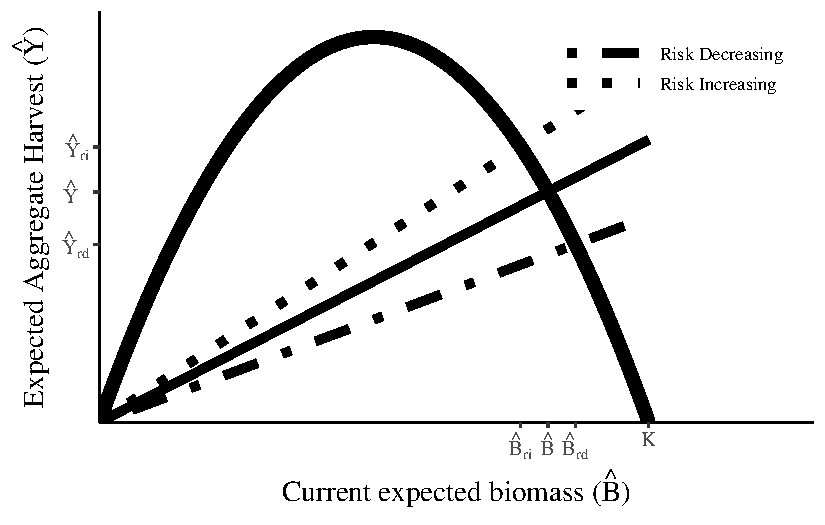
\includegraphics{ibi-behavior_files/figure-pdf/fig-synas-1.pdf}

}

\caption{\label{fig-synas}Expected steady state biomass and aggregate
harvest levels change with index insurance in common-pool fisheries. An
initial pre-insurance equilibrium exists at the intersection of the
growth curve and mean linear production (solid line). If the underlying
inputs are risk increasing the curve shifts to the left (dotted line)
with index insurance. If the underlying inputs are risk decreasing the
curve shifts to the right (dot-dash line) with index insurance.}

\end{figure}

Single variable aggregate effort measures are useful in
surplus-production models, but do not reflect the complexity of fisher
decisions. Asche \emph{et al.} (2020) demonstrates fishers often use
multiple inputs to harvest fish. Index insurance may raise or lower
individual inputs depending on their own unique risk effects, but the
overall direction of harvest decisions may not be so clear. Interactions
between the inputs could override effects of index insurance on
individual inputs. Little research has been done on multiple input
insurance models. Ramaswami (1993) only examined the total production
variance impacts on total harvest changes with insurance, but does not
elaborate on the response of specific inputs. The next section explores
how multiple inputs interact with each other and insurance to provide a
a more comprehensive picture of how index insurance will impact
fisheries.

\hypertarget{sec-multi}{%
\section{Insurance with multiple inputs}\label{sec-multi}}

We simplify the general model in Equation~\ref{eq-max} by using two
inputs, \(X\in\{{x_a,x_b}\}\) to better understand the impact of
insurance on multiple fishery inputs. Adding more variables complicates
the model without adding any additional insights. The complexities of
input interactions sufficiently arise with two inputs to demonstrate our
intended purpose.

The original specification of Just and Pope make no assumption on the
form of the second derivative of the risk effect function. We postulate
reasonable assumptions on the production risk function to assist with
comparative statics later on. The marginal impact of adding an input to
production variance should have diminishing effects, because it is
impossible to completely eliminate risk or experience infinite risks.
Therefore, when \(h_{x_a}(X)>0 \rightarrow h_{x_ax_a}(X)<0\), and when
\(h_{x_a}(X)<0 \rightarrow h_{x_ax_a}(X)>0\). The cross partial of risk
effects on production \(\frac{\partial h}{\partial x_a \partial x_b}\)
must also be flexible and depend on how inputs interact with each other.
For example, if adding an input does not contribute to the marginal risk
effect of another input then
\(\frac{\partial h}{\partial x_a \partial x_b}=0\). Inputs interactions
could be complementary in that adding a risk decreasing input further
enhances the risk reducing properties of the other inputs,
\(\frac{\partial h}{\partial x_a \partial x_b}>0\). In other instances
the inputs may interact counter actively in that adding more of a risk
increasing input might reduce the effect of a risk decreasing input,
\(\frac{\partial h}{\partial x_a \partial x_b}<0\). In principle, when
inputs share the same direction of risk effects, their cross partial
ought to be complementary, and when inputs have opposite risk effects
they will be counter productive.

We use the same insurance design from the previous section where
payouts, \(\gamma\), are triggered by \(\omega<0\), and we can partition
profit into good states and bad states. Fishers now maximize expected
utility by selecting two inputs.

\begin{equation}\protect\hypertarget{eq-max2}{}{
\begin{aligned}
U\equiv\max_{x_a,x_b}\mathbb{E}[U]=\int^{\infty}_{-\infty}&\left[ \int^{\bar\omega}_{-\infty}j_{\omega,\theta}(\omega,\theta)u(\pi(X,\hat{B},\theta,\omega)+(1-J(\bar\omega))\gamma)d\omega \right.\\
&\left.+\int^{\infty}_{\bar{\omega}}j_{\omega,\theta}(\omega,\theta) u(\pi(X,\hat{B},
\theta,\omega)-J(\bar\omega)\gamma)d\omega\right] d\theta
\end{aligned}
}\label{eq-max2}\end{equation}

Taking the first order conditions yields:

\begin{equation}\protect\hypertarget{eq-foc2}{}{
\begin{aligned}
\frac{\partial U}{\partial x_a}=&\int^{\infty}_{-\infty}\left[ \int^{\bar\omega}_{-\infty}j_{\omega,\theta}(\omega,\theta)u_{x_a}(\pi(X,\hat{B},\theta,\omega)+(1-J(\bar\omega))\gamma)\frac{\partial \pi}{\partial x_a}(X,\hat{B},\theta,\omega)d\omega\right.\\
&\left.+\int^{\infty}_{\bar{\omega}}j_{\omega,\theta}(\omega,\theta) u_{x_a}(\pi(X,\hat{B},\theta,\omega)-J(\bar\omega)\gamma)\frac{\partial \pi}{\partial x_a}(X,\hat{B},\theta,\omega)d\omega\right] d\theta\\
\frac{\partial U}{\partial x_b}=&\int^{\infty}_{-\infty}\left[ \int^{\bar\omega}_{-\infty}j_{\omega,\theta}(\omega,\theta)u_{x_b}(\pi(X,\hat{B},\theta,\omega)+(1-J(\bar\omega))\gamma)\frac{\partial \pi}{\partial x_b}(X,\hat{B},\theta,\omega)d\omega\right.\\
&\left.+\int^{\infty}_{\bar{\omega}}j_{\omega,\theta}(\omega,\theta) u_{x_b}(\pi(X,\hat{B},\theta,\omega)-J(\bar\omega)\gamma)\frac{\partial \pi}{\partial x_b}(X,\hat{B},\theta,\omega)d\omega\right] d\theta\\
\end{aligned}
}\label{eq-foc2}\end{equation}

Given the first order condition is satisfied, we can use the implicit
function theorem (IFT) to look at the impact of a change in the
exogenous insurance contract locally at the input solutions. Applying
IFT and Cramer's Rule yields a system of equations that determine the
impact of insurance on each optimal input:

\begin{equation}\protect\hypertarget{eq-ivtsol}{}{
\begin{aligned}
&\frac{\partial x_a}{\partial \gamma}=\frac{-1}{Det}\left[\frac{\partial U}{\partial x_b \partial x_b}\frac{\partial U}{\partial x_a \partial \gamma}-\frac{\partial U}{\partial x_a \partial x_b}\frac{\partial U}{\partial x_b \partial \gamma}\right] \\
&\frac{\partial x_b}{\partial \gamma}=\frac{-1}{Det}\left[\frac{-\partial U}{\partial x_b \partial x_a}\frac{\partial U}{\partial x_a \partial \gamma}+\frac{\partial U}{\partial x_a \partial x_a}\frac{\partial U}{\partial x_b \partial \gamma}\right]
\end{aligned}
}\label{eq-ivtsol}\end{equation}

Because the determinate will always be positive by the definition of the
second order condition, we can focus on the interior of the brackets. If
positive, then insurance will lower use of that specific input and vice
versa if negative. The partial derivatives are necessary to sign
Equation~\ref{eq-ivtsol}. Their complete derivations are included in the
appendix. The complex interaction between the partial effects of inputs
and insurance presents a challenge to understanding the impacts of index
insurance on fisheries. Therefore, we only focus on the uncorrelated
case where \(\theta\) and \(\omega\) are independent. Ambiguity already
exists with some level of basis risk. Introducing additional ambiguity
only obsurces insight further.

Specific conditions must be met to determine the overall impact of index
insurance on inputs, otherwise the effect could go either way despite
the risk increasing or decreasing characteristic of an individual input.

\begin{proposition}[]\protect\hypertarget{prp-samre}{}\label{prp-samre}

In fisheries with two inputs, when \(\theta\) and \(\omega\) are
uncorrelated, index insurance will change the optimal use of a specific
input in accordance to an input's own risk effect when the following
sufficient condition is true:

\(\frac{\partial U}{\partial x_a\partial x_b}>0\) when both inputs share
the same risk effects, and
\(\frac{\partial U}{\partial x_a\partial x_b}<0\) when inputs have
opposite risk effects.

Otherwise, Index Insurance will have ambiguous effects on optimal input
choice.

\end{proposition}

The proof is included in Section~\ref{sec-samre} and follows similar
steps as the proof of Proposition~\ref{prp-ind} while accounting for the
partial effects of each input.

Proposition~\ref{prp-samre} shows that index insurance can have clear
impacts on input use even in complex settings with multiple inputs
provided the sufficient condition holds. However, it is not clear
ex-ante what the sign of the cross partial inputs of the first order
condition should be. \(\frac{\partial U}{\partial x_a\partial x_b}\) and
\(\frac{\partial U}{\partial x_b\partial x_a}\) themselves could be
ambiguous. As shown in the appendix, rearranging
\(\frac{\partial U}{\partial x_a\partial x_b}\) and
\(\frac{\partial U}{\partial x_b\partial x_a}\) shows the relative
weight between the marginal profits of each input and the risk effects
cross partial influence the overall sign of first order cross partials.
Essentially, fishers change their inputs depending on whether a given
input makes the other input more productive than the risk it adds.
Whether inputs are complementary or counteractive in their risk effects
influence the sign of the cross partial. When inputs share risk effects,
they ought to increase the risk effects of each other. Therefore the
cross partial is more likely to be negative when inputs share risk
effects and positive when they are complementary following the
sufficient conditions proposed in Proposition~\ref{prp-samre}.

Even with two inputs, ambiguity on the optimal use exists. Extending to
more inputs introduces more interactions among the inputs, and the
relatively weighting between marginal productivity and the risk effect
cross partials is even harder to sign. Ramaswami (1993) used this
complexity as a justification to only examine the total variance of
production with a vector of inputs. Proposition~\ref{prp-samre} helps
elucidate his observations, while providing some understanding of how
different inputs could change when fishers use a variety of inputs.
Specific inputs could have different external environmental and
community impacts. Being better able to predict how index insurance
changes those inputs, and their ensuing impacts on a fishery, will help
minimize any negative impacts that could arise.

Despite the seemingly rigid conditions, Proposition~\ref{prp-samre}
provides useful insight into the behavioral effects insurance will have
when fishers use multiple inputs. It states that when the conditions
hold, the direction all inputs should change is based solely on the
characteristics of their own risk effects. Other inputs may influence
the magnitude of change, but the direction is unequivocal. It remains
unclear what the overall impacts on conservation will be in a multiple
input setting. Differences in mean production elasticity lead to
different magnitudes of change in input use. The overall change in
harvest, and thus conservation, depends on the aggregate change in
harvest. For example, a decline in use for a risk decreasing input
compared to an equivalent increase in use of a risk increasing input may
not lead to lower harvest if the risk increasing input is relatively
more productive.

The next section uses simulations to show the total impact on harvest
can vary substantially, and that the conditions to ensure unambiguous
input change can be met. Though when applied with real world estimates
of risk effects, the conditions may not hold and the effects of index
insurance does not follow simple rules.

\hypertarget{sec-sim}{%
\section{Numerical Simulations}\label{sec-sim}}

We use numerical simulation to show the ambiguity present in
Proposition~\ref{prp-corr}, test the necessary conditions in
Proposition~\ref{prp-samre}, and to determine the magnitude of change in
input use for Norwegian fisheries using the parameters found in Asche
\emph{et al.} (2020). Monte Carlo simulations find expected utility
across 1000 random draws of weather and biological variables. Constant
absolute risk aversion is used in each scenario to better account for
negative shocks and profit loss. A comprehensive parameters test the
sensitivity to different model parameters and the effects on optimal
input choices. All simulations are conducted in R with accompanying code
available at {[}WILL ADD ONCE REPO IS CLEANED{]}.

\hypertarget{simulations-with-biological-risk}{%
\subsection{Simulations with biological
risk}\label{simulations-with-biological-risk}}

We use the typical Just-Pope production structural form where
\(f(x)=x^\alpha\) and \(h(x)=x^\beta\). Mean production \(f(x)\) is
concave so that \(\alpha>0\). Risk effects on the input can either be
risk increasing or decreasing with \(\beta\lessgtr0\). We apply convex
costs, \(c(x)=cx^2\), for smoother convergence in the maximization
procedure. Biological and weather shocks are normally distributed with
\(\theta\sim N(0,\sigma_{\theta})\) and
\(\omega\sim N(0,\sigma_{\omega})\). The shocks are linked through a
copula with correlations ranging from \([0,1]\).

\begin{equation}\protect\hypertarget{eq-sim}{}{
\pi=x^\alpha(\hat\beta+\theta)+\omega x^\beta-cx^2
}\label{eq-sim}\end{equation}

Fishers will choose inputs \(x\) to maximize expected utility with an
insurance contract. Constant Absolute Risk Aversion (CARA) utility is
used to better account for negative shocks and profit loss.

\begin{equation}\protect\hypertarget{eq-maxsim}{}{
\begin{aligned}
U&\equiv\max_{x}\mathbb{E}[u]=\mathbb{E}[(1-\exp(-a(\pi(x,\hat\beta,\theta)+\mathbb{I}(\gamma))]\\
\mathbb{I}(\gamma)&=\begin{cases}-\rho\gamma & \text{if } \omega\ge \bar\omega\\
(1-\rho)\gamma & \text{if } \omega<\bar\omega
\end{cases}
\end{aligned}
}\label{eq-maxsim}\end{equation}

We convert \(\gamma\) to be a percentage of mean optimal profit without
insurance for interpretability. For example, \(\gamma=1\) would
represent full coverage of deviation from pre profit loss and
\(\gamma=0\) represents no insurance. The insurance contract is
triggered by \(\omega<\bar\omega\) and pays out \(\gamma\).

We create a wide parameter space to assess the sensitivity of optimal
input choices to different model parameters. We vary the relative
productivity of the input \(\alpha\in\{0.25,0.5,0.75\}\), the risk
effect of the input \(\beta\in\{-0.7,-0.5,-0.3,-0.1,0.1,0.3,0.5,0.7\}\),
the convexity of costs \(c\in\{0.1,0.2,0.3\}\), the risk aversion
parameter \(a\in\{1,2,3\}\), the biological shock variance
\(\sigma_{\theta}\in\{0.1,0.2,0.3,0.4\}\), the weather shock variance
\(\sigma_{\omega}\in\{0.1,0.2,0.3,0.4\}\), and the correlation between
the shocks \(\rho\in[0,1]\).

First we iterate \(\gamma\) from \(0\) to \(2\) to show the change in
optimal input use for a single input. Selected parameters for
Figure~\ref{fig-iter} are for demonstration purposes. The full parameter
space is explored in the accompanying code.

\begin{figure}

{\centering 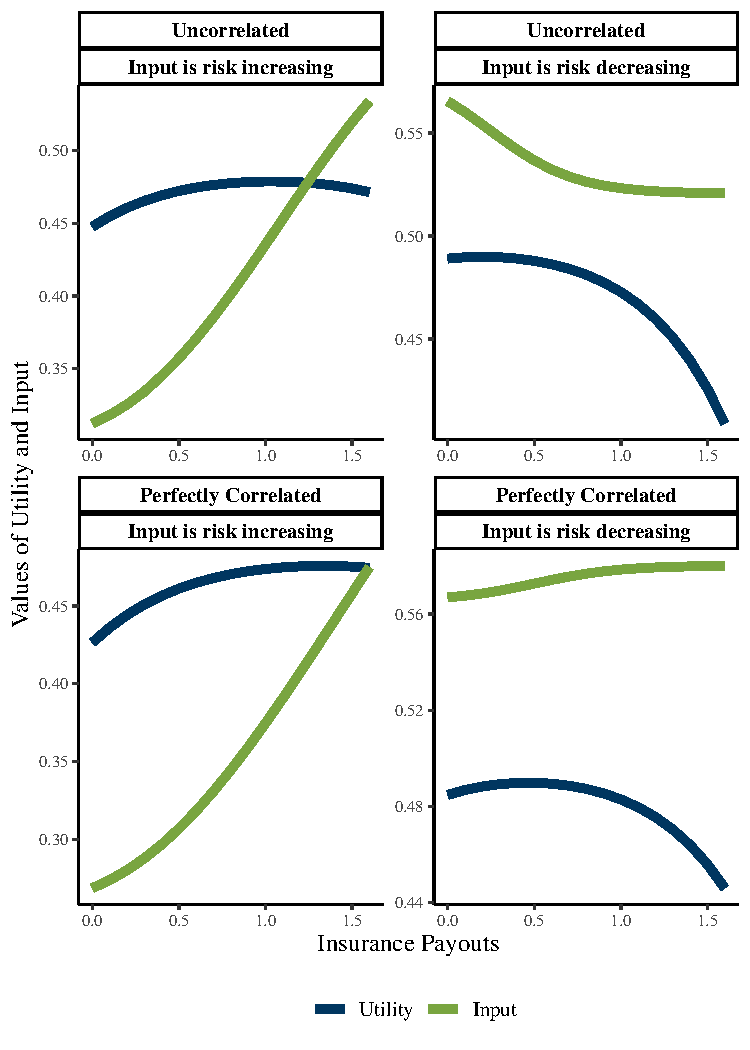
\includegraphics{ibi-behavior_files/figure-pdf/fig-iter-1.pdf}

}

\caption{\label{fig-iter}Improvements in utility (green lines) and
changes in optimal input use (blue lines) with index insurance. Shocks
are uncorrelated with high mean productivity (\(\alpha=0.75\)), high
risk aversion \(a=3\), and relatively more variable weather shocks than
biological (\(\sigma_{w}=0.4\) vs \(\sigma_{t}=0.1\))}

\end{figure}

Optimal input use changes monotonically with index insurance depending
on the risk characteristics of the input. Risk increasing inputs always
increase with insurance. Risk decreasing inputs are ambiguous following
Proposition~\ref{prp-ind} and Proposition~\ref{prp-corr}. When the
insured weather shocks are perfectly correlated with biological shocks,
the risk protection from insurance spills over to fishers encouraging
them take on more fish with expanded production.

The concavity of utility use implies there exists an optimal amount of
insurance for fishers to buy. An endogenous choice of \(\gamma\) will
also maintain the same sign of optimal input use because input use is
monotonic in \(\gamma\). However, the magnitudes of input use change
will depend on the level of \(\gamma\). Allowing fishers to choose
insurance coverage ensures that the choice of insurance and input use
changes are welfare improving and will not bias input choices with over
or under investment of insurance. Simulations moving forward will allow
fishers to choose both inputs and insurance coverage.

Adding this to Equation~\ref{eq-maxsim} amends the choice set:

\begin{equation}\protect\hypertarget{eq-maxsim2}{}{
\begin{aligned}
U&\equiv\max_{x,\gamma}\mathbb{E}[u]=\mathbb{E}[(1-\exp(-a(\pi(x,\hat\beta,\theta)+\mathbb{I}(\gamma))]\\
\mathbb{I}(\gamma)&=\begin{cases}-\rho\gamma & \text{if } \omega\ge \bar\omega\\
(1-\rho)\gamma & \text{if } \omega<\bar\omega
\end{cases}
\end{aligned}
}\label{eq-maxsim2}\end{equation}

Basis risk impacts the optimal choice of input, but the interaction
between the biological productivity and the risk effects of the input
are the primary drivers (Figure~\ref{fig-corr}). When mean productivity
is relatively low, basis risk has a negligible impact on the optimal
input use. Basis risk is more consequential at higher levels of mean
productivity. The trade off of less risk from insurance and loss of
income through lower production is far more salient. High risk
decreasing inputs see small levels of reduction when shocks are
uncorrelated. With less basis risk, fishers are willing to increase use
of risk decreasing inputs to capture more fish as insurance protects all
types of risk.

\begin{figure}

{\centering 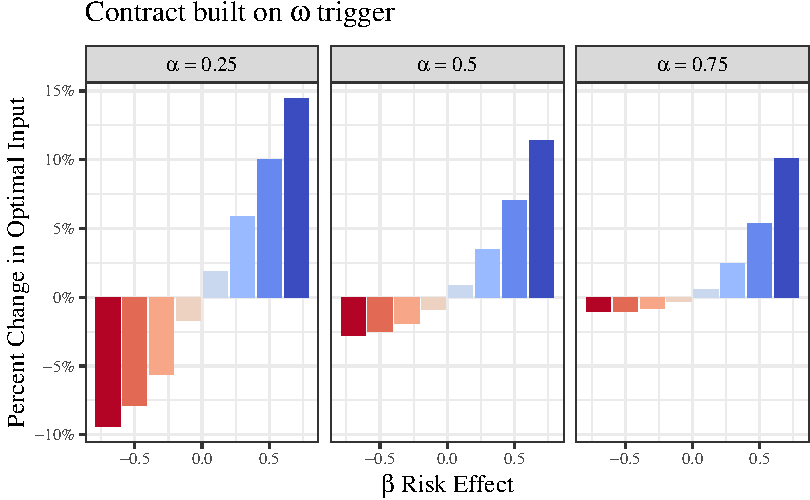
\includegraphics{ibi-behavior_files/figure-pdf/fig-corr-1.pdf}

}

\caption{\label{fig-corr}Percentage change in optimal input with an
index insurance contract. Risk increasing inputs (blue bars) always
increase input use, while risk decreasing inputs (red bars) have
ambiguous effects depending on the basis risk (correlation on the
x-axis) and relative productivity of the input (\(\alpha\) in the
panels).}

\end{figure}

Magnitude and sign of input change are sensitive to other parameters.
Figure~\ref{fig-sum} shows that on average, insurance decreases risk
decreasing input use by much smaller magnitudes than the proportional
rise in risk increasing input use. At moderate levels of mean
productivity, the average risk decreasing sees an increase for low
levels of risk aversion and low degrees of weather variation.

More risk averse fishers respond more aggressively to insurance and make
relatively more changes toward their input decisions (Panel A in
Figure~\ref{fig-sum}). Risk aversion implies more sensitivity towards
risk. The protection from insurance has greater marginal value for more
risk averse fishers. Greater marginal value of insurance means they can
invest less into risk reducing inputs than before, and have more
protection from greater shocks with risk increasing inputs.

Fisher input choice are much more responsive to insurance protection
from larger productivity risks (Panel B Figure~\ref{fig-sum}). Similar
to risk aversion, the greater the shocks the greater the marginal value
of insurance is to mitigate those shocks. In more volatile environments,
insurance provides significantly more income smoothing leading to
similar incentives as the higher risk aversion example.

Trigger levels do not appear to have differing impacts on input use.
Setting the trigger levels to more catastrophic coverage did not
encourage fishers to change their input use relative to the other
parameters. While necessary for applying Lemma~\ref{lem-mp} in the
proofs, the results of Proposition~\ref{prp-ind} and
Proposition~\ref{prp-corr} would appear to hold if \(\bar\omega\ne0\).

\begin{figure}

{\centering 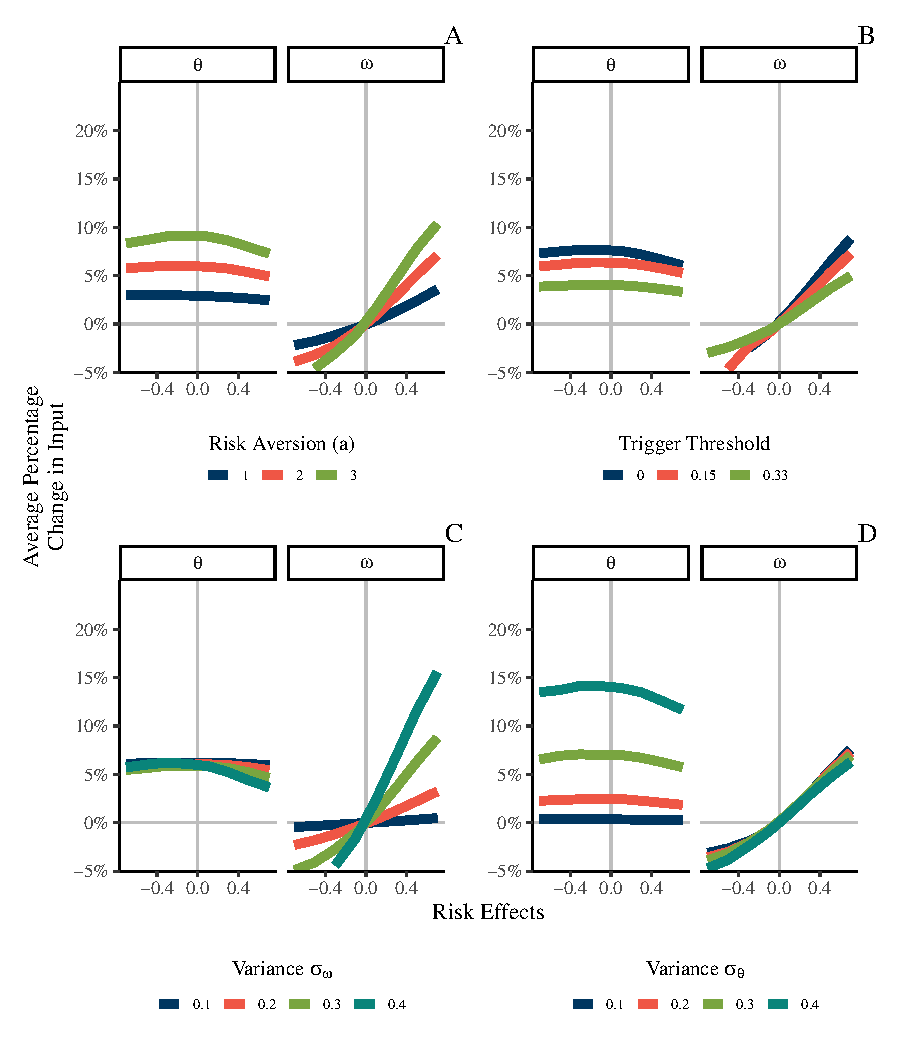
\includegraphics{ibi-behavior_files/figure-pdf/fig-sum-1.pdf}

}

\caption{\label{fig-sum}Risk Aversion (A), weather variance \(\omega\)
(B), and trigger (C) all influence the magnitude of change in harvest.
Mean production elasticity is set to 0.5. Average percent change in
input (y-axis) is summarized across all other parameter combinations for
each risk effect value of \(\beta\).}

\end{figure}

In the next section we use parameters from Asche \emph{et al.} (2020) to
calculate the overall change in harvest with multiple inputs interacting
with index insurance. These simulations will also show the conditions of
Proposition~\ref{prp-samre} do not hold in real world fisheries.

\hypertarget{application-to-real-world-fisheries}{%
\subsection{Application to Real World
Fisheries}\label{application-to-real-world-fisheries}}

Asche et al., (2020) aggregated by vessel type and not species, so there
is no reasonable estimate for biomass. They accounted for biomass using
fixed effects in their regression, but without additional information we
cannot parameterize the mean and variance of biomass. Therefore, our
simulations normalize mean biomass to 1 and we assume the biomass shocks
are uncorrelated with the risk fishers mitigate through \(h(X)\).
Norwegian fisheries are well managed so the biological variance could be
mitigated through quota systems or accurate stock assessments. The
simulation model uses three inputs instead of one.

\begin{equation}\protect\hypertarget{eq-sim3}{}{
\pi(k,l,f)=k^{\alpha_k}l^{\alpha_l}f^{\alpha_f}+\omega k^{\beta_k}l^{\beta_l}k^{\beta_f}-c_kk^2-c_ll^2-c_ff^2
}\label{eq-sim3}\end{equation}

Fishers in the simulation choose inputs and insurance coverage to
maximize expected utility.

\begin{equation}\protect\hypertarget{eq-maxasche}{}{
\begin{aligned}
U&\equiv\max_{\gamma,k,l,f}\mathbb{E}[u]=\mathbb{E}[u(k^{\alpha_k}l^{\alpha_l}f^{\alpha_f}+\omega k^{\beta_k}l^{\beta_l}k^{\beta_f}-c_kk^2-c_ll^2-c_ff^2+\mathbb{I}(\gamma)]\\
\mathbb{I}(\gamma)&=\begin{cases}-\rho\gamma & \text{if } \omega\ge \bar\omega\\
(1-\rho)\gamma & \text{if } \omega<\bar\omega
\end{cases}
\end{aligned}
}\label{eq-maxasche}\end{equation}

Table~\ref{tbl-asche} shows the production and risk elasticities of the
four vessel types used in the simulation. While not all elasticities
were found to be statistically different from zero, we used their raw
values because dropping only those variables that are significant in
both matching parameters would have kept only a few valid combinations.
All non-significant elasticities led to small changes as expected, but
their interactions with other inputs could partially drive some of the
observed outcomes.

\hypertarget{tbl-asche}{}
\begin{longtable}[]{@{}
  >{\raggedright\arraybackslash}p{(\columnwidth - 12\tabcolsep) * \real{0.2410}}
  >{\raggedleft\arraybackslash}p{(\columnwidth - 12\tabcolsep) * \real{0.1325}}
  >{\raggedleft\arraybackslash}p{(\columnwidth - 12\tabcolsep) * \real{0.1325}}
  >{\raggedleft\arraybackslash}p{(\columnwidth - 12\tabcolsep) * \real{0.1325}}
  >{\raggedleft\arraybackslash}p{(\columnwidth - 12\tabcolsep) * \real{0.1205}}
  >{\raggedleft\arraybackslash}p{(\columnwidth - 12\tabcolsep) * \real{0.1205}}
  >{\raggedleft\arraybackslash}p{(\columnwidth - 12\tabcolsep) * \real{0.1205}}@{}}
\caption{\label{tbl-asche}Production and Risk elasticities of Norwegian
Fisheries from Asche et al., (2020)}\tabularnewline
\toprule\noalign{}
\begin{minipage}[b]{\linewidth}\raggedright
\end{minipage} & \begin{minipage}[b]{\linewidth}\raggedleft
\(\alpha_k\)
\end{minipage} & \begin{minipage}[b]{\linewidth}\raggedleft
\(\alpha_l\)
\end{minipage} & \begin{minipage}[b]{\linewidth}\raggedleft
\(\alpha_f\)
\end{minipage} & \begin{minipage}[b]{\linewidth}\raggedleft
\(\beta_k\)
\end{minipage} & \begin{minipage}[b]{\linewidth}\raggedleft
\(\beta_l\)
\end{minipage} & \begin{minipage}[b]{\linewidth}\raggedleft
\(\beta_f\)
\end{minipage} \\
\midrule\noalign{}
\endfirsthead
\toprule\noalign{}
\begin{minipage}[b]{\linewidth}\raggedright
\end{minipage} & \begin{minipage}[b]{\linewidth}\raggedleft
\(\alpha_k\)
\end{minipage} & \begin{minipage}[b]{\linewidth}\raggedleft
\(\alpha_l\)
\end{minipage} & \begin{minipage}[b]{\linewidth}\raggedleft
\(\alpha_f\)
\end{minipage} & \begin{minipage}[b]{\linewidth}\raggedleft
\(\beta_k\)
\end{minipage} & \begin{minipage}[b]{\linewidth}\raggedleft
\(\beta_l\)
\end{minipage} & \begin{minipage}[b]{\linewidth}\raggedleft
\(\beta_f\)
\end{minipage} \\
\midrule\noalign{}
\endhead
\bottomrule\noalign{}
\endlastfoot
Coastal Seiners & 0.294 & 0.421 & 0.457 & 0.184 & -0.432 & 0.119 \\
Coastal Groundfish & 0.463 & 0.421 & 0.355 & 0.965 & -0.080 & 0.113 \\
Purse Seiners & 0.941 & -0.108 & 0.605 & -0.454 & -0.231 & 0.160 \\
Groundfish Trawlers & 0.210 & 0.106 & 0.531 & -2.788 & -0.110 &
-0.024 \\
\end{longtable}

Overall harvest changes from index insurance depend on interaction of
inputs, risk aversion, and the degree of varibilaity in the shocks.

\begin{figure}

{\centering 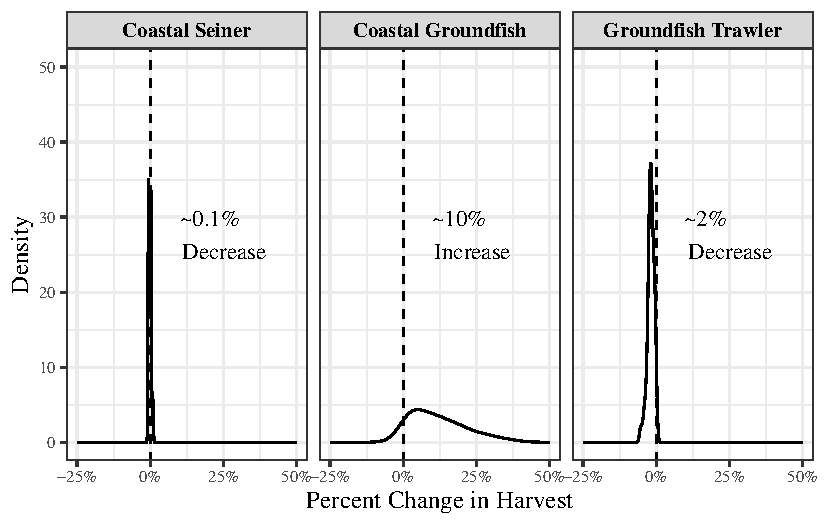
\includegraphics{ibi-behavior_files/figure-pdf/fig-asche-1.pdf}

}

\caption{\label{fig-asche}Density plots of the percent change in harvest
for each vessel type in Norwegian fisheries. The dashed line represents
no change in harvest. The text labels represent the median percent
change in harvest for each vessel type.}

\end{figure}

\begin{figure}

{\centering 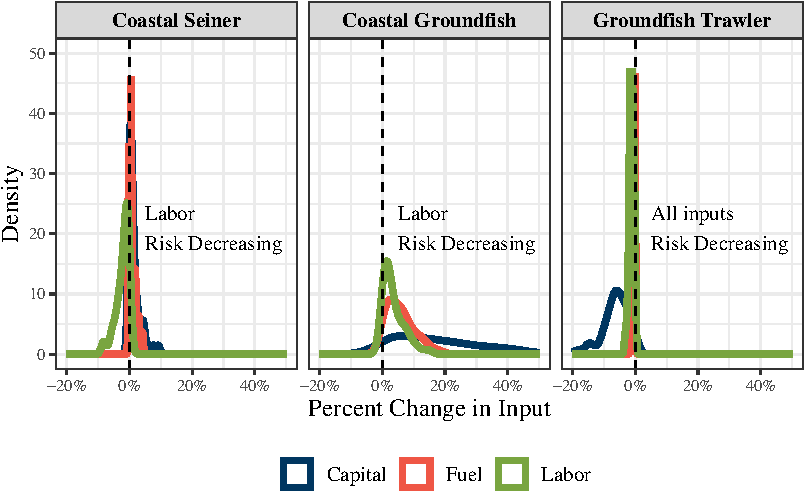
\includegraphics{ibi-behavior_files/figure-pdf/fig-asche-input-1.pdf}

}

\caption{\label{fig-asche-input}Density plots of the percent change in
input use for each vessel type in Norwegian fisheries. The dashed black
line represents no change in input use. Risk decreasing inputs are
labeled. Labor (green lines) is dropped for Purse Seiners because labor
was never used in simulations due to negative productivity elasticity.}

\end{figure}

Applying index insurance in Norwegian fisheries will lead to changes in
input use and overall harvest. Table~\ref{tbl-asche} shows that index
insurance leads to a wide range of possible harvest outcomes. The
coastal groundfish fishery observed the largest increase in harvest with
most simulations yielding around a 12.5\% increase in harvest. This was
driven primarily by increases capital (Figure~\ref{fig-asche-input}).
All inputs had relatively similar mean production elasticities, but
capital is strongly risk increasing with the highest positive risk
elasticity. Labor is a risk decreasing input, but also rises with
insurance. This is an example where the conditions of
Proposition~\ref{prp-samre} do not hold. The large discrepancy in
production risk elastiticites is probably a reason for this in addition
to the interactions terms at play by adding the third fuel input.

Purse seiners see the largest reduction in overall harvest, though
relatively small at only 4\%. Capital for purse seiners is the most
productive input out of all fisheries and inputs. Because it is risk
reducing, it dominates the slightly risk increasing fuel input to lead
the entire fishery to reduce harvest. This shows another case where the
conditions of Proposition~\ref{prp-samre} do not hold. Fuel use is risk
increasing, yet on average declines with index insurance. The ambiguity
of risk decreasing inputs remains present even in the strongest case.
While the median harvest decline is 4\%, there are still conditions with
high bioloigcal stochasticity and correlation that encourage fishers to
use more capital with insurance despite its risk decreasing nature.
Labor allocations did not change. No labor was allocated in either
optimal choice, because the production elasticity was negative.

Coastal seiners show the conditions for Proposition~\ref{prp-samre} can
hold in the real world with multiple inputs. In general, all input use
changes follow their respective risk effects. Capital (0.44\%) and fuel
(0.11\%) both increased, while labor (-1.01\%) decreased. In aggregate,
there was a small reduction in harvest (-0.3\%). While insurance led to
a change, it was rather small and would not have a large impact on the
fishery. The counteractive effects of the risk effects may negate some
of the desire to change production as insurance incentivizes both
increases and decreases in harvest.

Inputs in the groundfish trawler industry are all risk reducing.
Trawlers see a consistent 1.5\% decrease in harvest. Capital is
extremely risk reducing and is lower in nearly every simulation, but is
a relatively less productive input so overall harvest changes are small.

\hypertarget{sec-disc}{%
\section{Discussion}\label{sec-disc}}

Index insurance will have behavioral impacts on fishers' input
decisions, which in turn will lead to changes in fishery sustainability.
The direction and magnitude of impacts are primarily sensitive to the
risk effects of inputs used in production and can have ambiguous
outcomes. The traditional way of accounting for biological risk in
fishery models predicts that index insurance will always increase
fishing pressures. These models are inherently risk increasing and do
not adequately capture deeper risk mitigation strategies. Incorporating
more flexible production models that allow for both positive and
negative risk effects presents a more nuanced view of moral hazards in
fishery index insurance.

The fundamental driver of fishers' behavior changes is whether the
marginal change in productivity is balanced by the marginal change in
risk. Fishers are more willing to increase production if insurance
negates the additional risk of expanded production. When insurance
lowers risk, fishers need less self insurance through risk reducing
inputs and can reduce their use. However, using less inputs implies less
available catch and revenue creating a unique tension that exists
throughout our analysis. Across all simulations, decreased input use was
proportionally smaller than increased input use holding all other
parameters constant. Behavior change in fisheries will lean towards
expanding production creating a dilemma for conservation efforts.

As shown in this paper, harvest pressures could reduce by 4\% in
Norwegian purse seiners. Norwegian coastal groundfish trawlers were
incentivized to increase their harvest by 12.5\% with index insurance.
Without more specific biological information, we cannot extrapolate the
total effect on fish abundance. The magnitude of harvest change
indicates while index insurance may not be a conservation panacea in
isolation, it also may not be a destructive tool. The decision to
develop index insurance should revolve around whether it provides
sufficient financial relief for fishing communities when designed to
minimize negative impacts on fish stocks. While not the focal point of
this paper, the average gain in utility for Norwegian fishers from is
7\% indicating that index insurance can achieve welfare improving
outcomes for fishers moving forward.

Risk effects remain an elusive concept in fisheries and need to
reconciled in order to articulate more accurate behavior changes of
fishery index insurance. Crop covers and pesticide provide clear
examples of risk decreasing inputs in agriculture, but what do risk
decreasing inputs look like in fisheries? Asche \emph{et al.} (2020)
provide empirical evidence of the existence of risk decreasing inputs,
but do not elaborate on why or how labor and capital directly decrease
risk. Labor is perhaps the more intuitive risk decreasing input.
Technical expertise of crew and captains can hedge against luck when
fishing (Alvarez \emph{et al.} 2006). Better trained crew can deploy
gear in a safe and timely manner, increasing the likelihood of effective
sets.

Fuel as a risk increasing input in fisheries makes intuitive sense as
well. Fuel is used to power vessels and is a direct cost of fishing. The
more fuel used, the more fishing is occurring. The more fishing that is
occurring, the more risk is being taken on. Every hour at sea increases
the reward, but also the chances of failure.

Capital is a more complex input, because it can be both risk increasing
and decreasing. Capital investments in fisheries typically refer to
vessel tonnage, engine power, and gear technology. The spatiotemporal
dimension of fishing decisions may explain how capital can potentially
possess both risk effects. Fishers have to make decisions on where,
when, and how long to fish that differ from the set grids of agriculture
(Reimer \emph{et al.} 2017). Capital offers protection from risk by
allowing fishers to explore more fishing grounds, use more secure gear,
and fish in more adverse weather conditions. When common pool resources
incentivize the race to fish, having larger vessels may be a risk
reducing input as the sooner a fisher harvests from the stock, they
assure their income at the expense of other fishers. Adding risk
aversion to standard models of common pool fisheries suggests fishers
should lower their capital use compared to risk neutral allocations
(Mesterton-Gibbons 1993; Tilman \emph{et al.} 2018). Yet,
overcapitalization and overfishing are more often observed in the real
world. Either fishers are never risk averse or the risk effects of
capital are not as simple as the standard model suggests. When capital
is allowed to be risk decreasing, optimal input choices are much higher
than risk neutral equilibrium suggesting fishers are making rational,
risk averse decisions even while overfishing.

Biomass is a crucial fishery input that separates our analysis from
prior agricultural analyses. Most bioeconomic models simplify the
complex effects of stock dynamics into multiplicative forms as modeled
in this paper with \(f(X)\hat\beta+\theta\). However, different forms of
risk could be embedded into the biological component of fishery models.
Stock variance could be greater in overfished stocks instead of
healthier ones, reflecting more vulnerability in weaker states (Sims
\emph{et al.} 2018). The effects of insurance with these biological risk
effects could lead to unique changes in fisher behavior. If insurance
protects from more risk, fishers may be more willing to expose
themselves to greater risk at more vulnerable stock levels.
Alternatively, insurance could help mitigate risk and incentivize
fishers to move toward healthier stocks with less variance by
alleviating pressures to fish. Further analysis is required to
understand the full implications of biological risk effects in
fisheries.

The transfer between inputs and insurance reflects the substitution
between self-insurance and formal insurance (Quaas and Baumgärtner
2008). If index insurance is designed to reduce fishing capacity,
efforts must be made to ensure that it does not take away from the self
resiliency of fishers. Labor appears to be consistently risk reducing
and acts as a form of self insurance. If index insurance incentivizes
captains to hire less crew, the stock of fish may be preserved, but less
employment may reverberate throughout the community. Fishing is often a
primary employment opportunity in coastal communities. Lowering
employment options may lead to increased poverty or concentrated wealth.
The resiliency of the community would be compromised rather than
enhanced. The same idea applies to capital. If fishers are over
investing in capital to hedge against some form of risk, policymakers
need to be sure the insurance is replacing maladaptive self insurance
behavior.

The primary form of self insurance in fisheries is management. To this
point our analysis explicitly modeled scenarios without the existence of
management. Most fisheries are managed in some form. The interaction
between management and insurance may be complementary or substitutes.
For example, well managed fisheries that have responsive harvest control
rules may not need insurance. The management system is already providing
the necessary risk protection. Insurance demand and uptake may be low in
these fisheries. Insurance could instead complement management to
provide the financial relief that management cannot offer. Managers
often focus on the biological health of the fishery that can run at odds
with fishers' desires to enhance their income. Insurance can act as the
financial relief and allow managers to pursue more active strategies to
protect fish stocks without political resistance from lowered quotas.
The interaction between insurance and management requires further
investigation especially with the the numerous management strategies
that exist in fisheries.

Design and access of insurance must also consider equity. The current US
federal disaster relief program is inequitable with bias towards large
industrial vessels (Jardine \emph{et al.} 2020). Creating another
program with equal inequity would be foolhardy. Current US farm
subsidies, including insurance premiums, are heavily skewed towards
large agribusinesses (White and Hoppe 2012). Dimensions of access,
procedural, representation, and distribution must all be built into the
design of new fishery index insurance programs (Fisher \emph{et al.}
2019). For example, small scale fishers may have income constraints that
prevent them from buying the initial contract. Micro-finance options
connected to insurance have been used in agriculture to alleviate this
burden with some success (Dougherty \emph{et al.} 2021). Additionally,
we must ensure that is not only the vessel owners who reap the benefits
of insurance. Deckhands and crew are laid off during closures. If index
insurance payouts are going through the entire fishery, the most
vulnerable to closures must be protected as well. Contract stipulations
could mandate that only cost expenses are covered by payouts thereby
including lost wages to the crew. Agriculture contracts often are
designed to directly cover expenses. Labor expenses could be included in
the contract to ensure that the crew is protected as well.

Our model only directly models behavior change through moral hazards.
Index insurance could be designed to incentivize other forms of
sustainable behavior change. We define three pathways insurance can
change behavior: Moral hazards, Quid Pro Quo, and Collective Action.
Moral hazards were proven in this paper to have ambiguous impacts
controlled by the risk characteristics of fishery inputs.

Quid Pro Quo expands contract design to explicitly build in conservation
measures. Fishers would be required to adopt sustainable practices in
order to qualify for insurance. Quid Pro Quo is already used in
agricultural insurance in the form of Good Farm Practices. Farmers must
submit management plans to US Risk Management Agency that clearly
outline their conservation practices in order to qualify for insurance.
Working closely with management agencies, insurance companies could
design contracts that require fishers to follow fishery specific
management practices. For example, fishers may be incentivized to use
more sustainable gear types, have an observer onboard, or reduce
bycatch. Manager input is needed to tailor fishery best practices to
insurance contracts. Further research would need to uncover the full
impact of Quid Pro Quo, but an initial hypothesis would be the fishers
will be willing to adopt sustainable practices so long as the marginal
gain in utility from the insurance is greater or equal to the necessary
sustainable changes. Otherwise fishers will not want to buy the
contracts and the insurance has no binding stipulations to change the
fishery.

Collective action ties insurance premiums to biological outcomes to
leverage the political economy of the fishery. Insures could reduce
premiums in fisheries that have robust management practices such as
adaptive harvest control rules, stock assessments, or marine protected
areas in the vicinity. Fishers could either pressure regulators to adopt
these actions or form industry groups to undertake the required actions.
Insurers would agree to this if triggers are connected to biological
health so that negative shocks are less frequent and thus payouts occur
less. Fishers gain from the reduced insurance premium and the increased
sustainability of harvest with rigorous management in place.

Ultimately, if index insurance is to be used in fisheries, it must be
designed with clear objectives and intentions. Index insurance can meet
objectives of income stability and risk reduction. There has been an
implicit assumption by practitioners that index insurance will always
lead to improved sustainability. Without considering the behavior change
of fishers when adopting insurance, the outcomes may not be as expected.
New insights derived from this paper will help guide the efficient and
sustainable implementation of fisheries index insurance.

\newpage
\appendix
\renewcommand{\thefigure}{A\arabic{figure}}
\renewcommand{\thetable}{A\arabic{table}}
\setcounter{figure}{0}
\setcounter{table}{0}

\hypertarget{appendix}{%
\section{Appendix}\label{appendix}}

\hypertarget{proof-of-lem-mp}{%
\subsection{\texorpdfstring{Proof of
Lemma~\ref{lem-mp}}{Proof of Lemma~}}\label{proof-of-lem-mp}}

\textbf{Lemma 3.1} \emph{Individual fisher expected marginal profit of a
specific input, \(x_m\), is greater in the good state than expected
marginal profit in the bad state when \(h_{x_m}(X^i)>0\). Expected
marginal profit is higher in the bad state when \(h_{x_m}(X^i)<0\). If
\(h_{x_m}(X^i)=0\), the marginal profits are equivalent in both states.}

By the first order conditions, there exist optimal values of any
individual input \(x_m^{i*}\) that must be chosen before the realization
of the states of the world. Therefore \(h(X^{i*})\), \(f(X^{i*})\), and
\(c(X^{i*})\) are equal across states.

Marginal utility in both states of the world is controlled by risk
effects and the sign of the random variable \(\omega\). Risk increasing
inputs have \(h_x'(X)>0\) by definition. For any input denoted by \(x\)
this holds \begingroup\makeatletter\def\f@size{7}\check@mathfonts
\begin{equation}\protect\hypertarget{eq-comppi1}{}{
\begin{aligned}
\small
\frac{\partial \mathbb{E}[\pi^i|\omega<\bar\omega]}{\partial x^{i*}_m}-\frac{\partial \mathbb{E}[\pi^i|\omega>\bar\omega]}{\partial x^{i*}_m}=&\mathbb{E}[\omega h_{x_m^*}(X^{i*})|\omega<\bar\omega]+\cancel{f_{x_m^*}(X^{i*})\hat{B}(X^{i*},Y(X^{\sim j *}))}+\cancel{f_{x^*_m}(X^{i*})[\frac{\partial \hat{B}}{\partial x_m^{*}}+\frac{\partial B}{\partial Y(X^{\sim j*})}\frac{\partial Y(X^{\sim j *})}{\partial x^*_m}]}-\cancel{c_{x^*_m}(X^{i*})} \\
&-\mathbb{E}[\omega h_{x_m^*}(X^{i*})|\omega>\bar\omega]+\cancel{f_{x_m^*}(X^{i*})\hat{B}(X^{i*},Y(X^{\sim j *}))}+\cancel{f_{x^*_m}(X^{i*})[\frac{\partial \hat{B}}{\partial x_m^{*}}+\frac{\partial B}{\partial Y(X^{\sim j*})}\frac{\partial Y(X^{\sim j *})}{\partial x^*_m}]}-\cancel{c_{x^*_m}(X^{i*})} \\
=&\mathbb{E}[\omega h_{x_m^*}(X^{i*})|\omega<\bar\omega]-\mathbb{E}[\omega h_{x_m^*}(X^{i*})|\omega>\bar\omega]
\end{aligned}
}\label{eq-comppi1}\end{equation}

\endgroup

If an input is risk decreasing then \(h_{x_m}(X^i)<0\). Then
Equation~\ref{eq-comppi1} is positive and marginal profit in the bad
state is greater than the marginal profit in the good state. Adding more
of a risk reducing input reduces the negative impact in the bad state
relative to the good state.

\[
\frac{\partial \mathbb{E}[\pi^i|\omega<\bar\omega]}{\partial x^{i*}_m}-\frac{\partial \mathbb{E}[\pi^i|\omega>\bar\omega]}{\partial x^{i*}_m}=\overbrace{\mathbb{E}[\omega h_{x_m^*}(X^{i*})|\omega<\bar\omega]-\mathbb{E}[\omega h_{x_m^*}(X^{i*})|\omega>\bar\omega]}^{+}
\]

Repeating the same thing for risk increasing inputs \(h_{x_m}(X^i)>0\)
shows that marginal profit in the bad state is less than marginal profit
in the good state.

\[
\frac{\partial \mathbb{E}[\pi^i|\omega<\bar\omega]}{\partial x^{i*}_m}-\frac{\partial \mathbb{E}[\pi^i|\omega>\bar\omega]}{\partial x^{i*}_m}=\overbrace{\mathbb{E}[\omega h_{x_m^*}(X^{i*})|\omega<\bar\omega]-\mathbb{E}[\omega h_{x_m^*}(X^{i*})|\omega>\bar\omega]}^{-}
\]

If inputs have no risk effects then \(h_{x_m}(X^i)=0\). Subbing into
Equation~\ref{eq-comppi1} shows there is no difference in marginal
profits with no risk effects.

\hypertarget{sec-partial}{%
\subsection{Partial derivatives}\label{sec-partial}}

Partial derivatives used to sign Equation~\ref{eq-ivtsol} are shown
below.

\begin{equation}\protect\hypertarget{eq-kk}{}{
\begin{aligned}
\frac{\partial F}{\partial k \partial k}&=(1-p)u''(\pi_g-p\gamma)(\frac{\partial \pi_g}{\partial k})^2+(1-p)u'(\pi_g-p\gamma)\frac{\partial^2 \pi_g}{\partial k\partial k}\\
&+ pu''(\pi_b+(1-p)\gamma)(\frac{\partial \pi_b}{\partial k})^2+pu'(\pi_b+(1-p)\gamma)\frac{\partial^2 \pi_b}{\partial k \partial k}
\end{aligned}
}\label{eq-kk}\end{equation}

\begin{equation}\protect\hypertarget{eq-ll}{}{
\begin{aligned}
\frac{\partial F}{\partial l \partial l}&=(1-p)u''(\pi_g-p\gamma)(\frac{\partial \pi_g}{\partial l})^2+(1-p)u'(\pi_g-p\gamma)\frac{\partial^2 \pi_g}{\partial l\partial l}\\
&+ pu''(\pi_b+(1-p)\gamma)(\frac{\partial \pi_b}{\partial l})^2+pu'(\pi_b+(1-p)\gamma)\frac{\partial^2 \pi_b}{\partial l \partial l}
\end{aligned}
}\label{eq-ll}\end{equation}

\begin{equation}\protect\hypertarget{eq-crossl}{}{
\begin{aligned}
\frac{\partial F}{\partial k \partial l}&=(1-p)u''(\pi_g-p\gamma)\frac{\partial \pi_g}{\partial k}\frac{\partial \pi_g}{\partial l}+(1-p)u'(\pi_g-p\gamma)\frac{\partial \pi_g}{\partial k\partial l}\\
&+ pu''(\pi_b+(1-p)\gamma)\frac{\partial \pi_b}{\partial k}\frac{\partial \pi_b}{\partial l}+pu'(\pi_b+(1-p)\gamma)\frac{\partial \pi_b}{\partial k \partial l}
\end{aligned}
}\label{eq-crossl}\end{equation}

\begin{equation}\protect\hypertarget{eq-crossk}{}{
\begin{aligned}
\frac{\partial F}{\partial l \partial k}&=(1-p)u''(\pi_g-p\gamma)\frac{\partial \pi_g}{\partial l}\frac{\partial \pi_g}{\partial k}+(1-p)u'(\pi_g-p\gamma)\frac{\partial \pi_g}{\partial l\partial k}\\
&+ pu''(\pi_b+(1-p)\gamma)\frac{\partial \pi_b}{\partial l}\frac{\partial \pi_b}{\partial k}+pu'(\pi_b+(1-p)\gamma)\frac{\partial \pi_b}{\partial l \partial k}
\end{aligned}
}\label{eq-crossk}\end{equation}

\begin{equation}\protect\hypertarget{eq-kgam}{}{
\frac{\partial F}{\partial k \partial \gamma}=(1-p)u''(\pi_g-p\gamma)\frac{\partial \pi_g}{\partial k}(-p)+pu''(\pi_b+(1-p)\gamma)\frac{\partial \pi_b}{\partial k}(1-p)
}\label{eq-kgam}\end{equation}

\begin{equation}\protect\hypertarget{eq-lgam}{}{
\frac{\partial F}{\partial l \partial \gamma}=(1-p)u''(\pi_g-p\gamma)\frac{\partial \pi_g}{\partial l}(-p)+pu''(\pi_b+(1-p)\gamma)\frac{\partial \pi_b}{\partial l}(1-p)
}\label{eq-lgam}\end{equation}

\hypertarget{sec-samre}{%
\subsection{\texorpdfstring{Proof of
Proposition~\ref{prp-samre}}{Proof of Proposition~}}\label{sec-samre}}

\begin{proof}

Lemma~\ref{lem-mp} allows us to sign the partial equations
\(\frac{\partial U}{\partial x^i_a\partial \gamma}\) and
\(\frac{\partial U}{\partial x^i_b\partial \gamma}\)
(Equation~\ref{eq-kgam} and Equation~\ref{eq-lgam} in the appendix) for
any risk effect on either input. Concave utility by definition leads to
\(u_{xx}<0\). For simplicity, we will only focus on
\(\frac{\partial U}{\partial x^i_a\partial \gamma}\), but all applies
equally to \(\frac{\partial U}{\partial x^i_b\partial \gamma}\).
Insurance payouts equalize profits between different states. If
insurance completely covers all loss and \(x^i_a\) is risk increasing,
then \(\frac{\partial U}{\partial x_a\partial \gamma}\) is positive.

\begin{equation}\protect\hypertarget{eq-kgamsol}{}{
\frac{\partial U}{\partial x_a \partial \gamma}=\overbrace{\overbrace{(1-F(\bar\omega))u_{x_ax_a}(\cdot)}^{-}\overbrace{[\frac{\partial \mathbb{E}[\pi^i|w<\bar\omega]}{\partial x_a}-\frac{\partial \mathbb{E}[\pi^i|w>\bar\omega]}{\partial x_a}]}^{-}}^{+}
}\label{eq-kgamsol}\end{equation}

Suppose both inputs are risk increasing so
\(\frac{\partial U}{\partial x^i_a\partial \gamma}\) and
\(\frac{\partial U}{\partial x^i_b\partial \gamma}\) are positive. The
only way for Equation~\ref{eq-ivtsol} to be unambiguously positive is
for \(\frac{\partial U}{\partial x^i_a\partial x^i_b}\) and
\(\frac{\partial U}{\partial x^i_a\partial x^i_b}\)
(Equation~\ref{eq-crossl} and Equation~\ref{eq-crossk} in the appendix)
to be positive.

\[
\begin{aligned}
&\frac{\partial x^i_a}{\partial \gamma}=\overbrace{\frac{-1}{Det}}^{-}\left[\overbrace{\overbrace{\frac{\partial U}{\partial x^i_b \partial x^i_b}}^{-}\overbrace{\frac{\partial U}{\partial x^i_a \partial \gamma}}^{+}\overbrace{-\frac{\partial U}{\partial x^i_a \partial x^i_b}}^{-}\overbrace{\frac{\partial U}{\partial x^i_b \partial \gamma}}^{+}}^{-}\right] >0\\
&\frac{\partial x^i_b}{\partial \gamma}=\overbrace{\frac{-1}{Det}}^{-}\left[\overbrace{\overbrace{\frac{-\partial U}{\partial x^i_b \partial x^i_a}}^{-}\overbrace{\frac{\partial U}{\partial x^i_a \partial \gamma}}^{+}+\overbrace{\frac{\partial U}{\partial x^i_a \partial x^i_a}}^{-}\overbrace{\frac{\partial U}{\partial x^i_b \partial \gamma}}^{+}}^{-}\right]>0
\end{aligned}
\]

Both risk increasing inputs will be raised with index insurance.
Repeating the same steps above with risk decreasing inputs shows both
inputs unambiguously decrease with index insurance.

Now suppose inputs have mixed risk effects. For simplicity, \(x^i_a\)
will be risk increasing and \(x^i_b\) will be risk decreasing. The
results will hold for the opposite case. By Lemma~\ref{lem-mp},
\(\frac{\partial U}{\partial x^i_a\partial \gamma}\) is positive, while
\(\frac{\partial U}{\partial x^i_b\partial \gamma}\) is negative.
Equation~\ref{eq-ivtsol} will be unambiguously positive if
\(\frac{\partial U}{\partial x^i_a\partial x^i_b}\) and
\(\frac{\partial U}{\partial x^i_b\partial x^i_a}\) are negative.

\[
\begin{aligned}
&\frac{\partial x^i_a}{\partial \gamma}=\overbrace{\frac{-1}{Det}}^{-}\left[\overbrace{\overbrace{\frac{\partial U}{\partial x^i_b\partial x^i_b}}^{-}\overbrace{\frac{\partial U}{\partial x^i_a \partial \gamma}}^{+}\overbrace{-\frac{\partial U}{\partial x^i_a \partial x^i_b}}^{+}\overbrace{\frac{\partial U}{\partial x^i_b\partial \gamma}}^{-}}^{-}\right] >0\\
&\frac{\partial x^i_b}{\partial \gamma}=\overbrace{\frac{-1}{Det}}^{-}\left[\overbrace{\overbrace{\frac{-\partial U}{\partial x^i_b\partial x^i_a}}^{+}\overbrace{\frac{\partial U}{\partial x^i_a \partial \gamma}}^{+}+\overbrace{\frac{\partial U}{\partial x^i_a \partial x^i_a}}^{-}\overbrace{\frac{\partial U}{\partial x^i_b\partial \gamma}}^{-}}^{+}\right]<0
\end{aligned}
\]

The risk increasing input will be raised with index insurance, while the
risk decreasing input will be lowered.

If these conditions do not hold, then it is impossible to determine
which additive element outweighs the other, and the insurance effects on
optimal input use will be ambiguous regardless of the underlying risk
effects of an input.

\end{proof}

\hypertarget{cross-partial-comparison}{%
\subsection{Cross partial comparison}\label{cross-partial-comparison}}

Dividing \(\frac{\partial F}{\partial k\partial l}\) by
\(-\frac{u'}{u'}\) allows us to rearrange terms to show the tension
between mean production and risk effects.

\begin{equation}\protect\hypertarget{eq-crosssolve}{}{
\begin{aligned}
-\frac{\partial F}{\partial k \partial l}&=(1-p)u'\frac{-u''}{u'}\frac{\partial \pi_g}{\partial k}\frac{\partial \pi_g}{\partial l}-(1-p)u'\frac{\partial \pi_g}{\partial k\partial l}\frac{u'}{u'}\\
&+ pu'\frac{\partial \pi_b}{\partial k}\frac{\partial \pi_b}{\partial l}\frac{-u''}{u'}-pu'\frac{\partial \pi_b}{\partial k \partial l}\frac{u'}{u'}\\
&=(1-p)u'[\frac{-u''}{u'}]\frac{\partial \pi_g}{\partial k}\frac{\partial \pi_g}{\partial l}+pu'[\frac{-u''}{u'}]\frac{\partial \pi_b}{\partial k}\frac{\partial \pi_b}{\partial l}\\
&-(1-p)u'\frac{\partial \pi_g}{\partial k\partial l}-pu'\frac{\partial \pi_b}{\partial k \partial l}
\end{aligned}
}\label{eq-crosssolve}\end{equation}

The concavity of profit with positive risk aversion \(\frac{-u''}{u'}\)
lead line 3 in Equation~\ref{eq-crosssolve} to be positive. The cross
partials in line 4 paint a more complicated picture. Whether inputs
enhance or reduce the risk effect qualities of each other influences the
weight of line 4. When inputs share risk effects, they ought to increase
the risk effects of each other so that
\(\frac{\partial h}{\partial k \partial l}>0\). Therefore line 4 in
Equation~\ref{eq-crosssolve} becomes more negative as all terms are
positive. It is relatively more likely that Equation~\ref{eq-crosssolve}
is negative when risk effects are shared.

When risk effects are mixed, with one input increasing and one input
decreasing, the risk effects counteract each other
\(\frac{\partial h}{\partial k \partial l}<0\). Line 4 in
Equation~\ref{eq-crosssolve} becomes relatively less negative. If the
difference between the risk effects cross partial
\(\frac{\partial h}{\partial k \partial l}\) outweigh the mean
production cross partial \(\frac{\partial f}{\partial k \partial l}\)
then line 4 becomes unambiguously becomes positive. Then
\(-\frac{\partial F}{\partial k \partial l}>0\) and
\(-\frac{\partial F}{\partial l \partial k}>0\). The relative changes
with complimentary or counteractive risk effects matches the signs
needed for the condition in Proposition~\ref{prp-samre} to hold.

\hypertarget{extra-proofs}{%
\subsection{Extra proofs}\label{extra-proofs}}

\begin{proposition}[]\protect\hypertarget{prp-rn}{}\label{prp-rn}

Risk neutral fishers will not change their input use with index
insurance

\end{proposition}

\begin{proof}

Risk neutrality implies that \(u'(k,l)=0\) and \(u''(k,l)=0\). Subbing
\(u''(k,l)=0\) into both Equation~\ref{eq-kgam} and
Equation~\ref{eq-lgam} forces them to both equal zero. Plugging zero for
\(\frac{\partial F}{\partial l \partial \gamma}\) and
\(\frac{\partial F}{\partial k \partial \gamma}\) into
Equation~\ref{eq-ivtsol} makes both elements also zero in the interior.
Thus risk neutral fishers would not change input allocation with the
addition of index insurance.

\end{proof}

\begin{proposition}[]\protect\hypertarget{prp-rezero}{}\label{prp-rezero}

Index insurance will not change the input allocations when all inputs
possess no risk effects.

\end{proposition}

\begin{proof}

The second part of Lemma~\ref{lem-mp} states that the marginal profits
across states are equal. If the marginal profits across states are
equal, then in Equation~\ref{eq-kgam} and Equation~\ref{eq-lgam} the
weight between positive and negative utilities is also equal and cancel
out leading to Equation~\ref{eq-kgam} and Equation~\ref{eq-lgam} both
equaling zero. Plugging zeros into Equation~\ref{eq-ivtsol} for the
insurance partials leads to an interior zero and no change in input use.

\end{proof}

Risk averse fishers will buy actuarially fair insurance. If the inputs
possess risk effects then they will lead to changes in the input.
Proposition~\ref{prp-samre} defines the change in multiple inputs
simultaneously with insurance.

\hypertarget{sec-simres}{%
\subsection{Multiple Input simulation results}\label{sec-simres}}

First, we present the simulations from the two input case to gain
additional insight into how index insurance changes multiple inputs.
Fishers earn profit through harvest with a Just and Pope production
function with mean biomass normalized to one, and convex cost function.
Inputs \(X \in \{x_a,x_b\}\) are replaced with capital (\(k\)) and labor
(\(l\)) to ground the interpretation of results in inputs practically
used by fishers.

\begin{equation}\protect\hypertarget{eq-sim}{}{
\pi(k,l)=\hat{B}k^{\alpha_k}l^{\alpha_l}+\omega k^{\beta_k}l^{\beta_l}-c_kk^2-c_ll^2
}\label{eq-sim}\end{equation}

Random shocks (\(\omega\)) are distributed normally with a mean of zero
and a standard deviation of \(\sigma_w\). Capital (\(k\)) and labor
(\(l\)) have both mean production elasticities (\(\alpha_k\) and
\(\alpha_l\)) and flexible risk elasticities (\(\beta_k\) and
\(\beta_l\)). Fishers choose both capital and labor to maximize expected
utility with constant absolute risk aversion (CARA).

Multiple index insurance policies are tested through changes in coverage
and trigger levels. One scenario sets an exogenous constant payout
amounts between 0-200\% of pre-insurance profit, and the other allows
fishers to endogenously choose payouts. The theoretical results of
Section~\ref{sec-common} and Section~\ref{sec-multi} provide comparative
statics on \(\gamma\) payouts as a means to test whether some insurance
is preferred to no insurance and how input use would change. Since the
sign remains the same for any \(\gamma\), the endogenous choice will
also maintain the same sign. However, the magnitudes of input use change
will depend on the level of \(\gamma\). Allowing fishers to choose
insurance coverage ensures that the choice of insurance and input use
changes are welfare improving and will not bias input choices with over
or under investment of insurance.

Trigger levels are set to engage at any below average weather or for
shocks of more than 75\% loss. All premiums are actuarilly fair. Risk
effects vary between -0.7 and 0.7 with iterative increases of 0.1
ignoring situations of 0 risk effects. Fishers can posses low, medium,
and high mean production elasticity values
\(\alpha\in\{0.25,0.5,0.75\}\). Coefficient of constant absolute risk
aversion ranges from 1 to 3. Within each scenario, a Monte Carlo
simulation creates 1000 weather random weather shocks with three
variants of standard deviation \(\sigma_w\in\{0.33,0.5,1\}\).

Increasing insurance incentivizes fishers to use more risk decreasing
inputs and less risk increasing inputs (Figure~\ref{fig-ins}). These
results confirm Proposition~\ref{prp-samre}, and show the conditions of
Proposition~\ref{prp-samre} can be satisfied with CARA utility and a
Just-Pope Production function (Figure~\ref{fig-ins}). The direction of
input use is also stable as each class of input is monotonically
increasing or decreasing with more insurance coverage. Inputs follow
expected changes in use given their own risk effect even when risk
effects are mixed. Capital is risk decreasing in the bottom left panel
and decreases with more insurance while the risk increasing labor
increases. The opposite trend occurs in the top right panel. The case
where both inputs are risk increasing mimics traditional fishery models
and shows that insurance will always increase input use.

Index insurance also increases utility shown by the green lines in
Figure~\ref{fig-ins}, but there exists an optimal amount of insurance
coverage for fishers. The optimal values of insurance are generally
lower when fishers use risk decreasing inputs. Notice the peak of the
green line in the bottom right quadrant of Figure~\ref{fig-ins} is
closer to 0 than that of the top left quadrant. Even in the mixed case,
the optimal amount of coverage is lower than when both inputs are risk
increasing. Risk decreasing inputs and insurance act as substitutes for
each other as they both lower fisher income variance. Risk decreasing
inputs still contribute to production while simultaneously reducing
variance. Insurance lowers the need of risk decreasing inputs for their
risk reduction qualities, but cannot fully compensate for the foregone
production. Thus, fishers will choose to use insurance until the
opportunity cost of lost marginal production is equal to insurance gains
in marginal risk protection.

Fishers are more willing to use risk increasing inputs with insurance
because the insurance protects from the added risk of more inputs.
Purchasing more insurance provides greater protection creating a
feedback loop that greatly expands productive input use.

\begin{figure}

{\centering 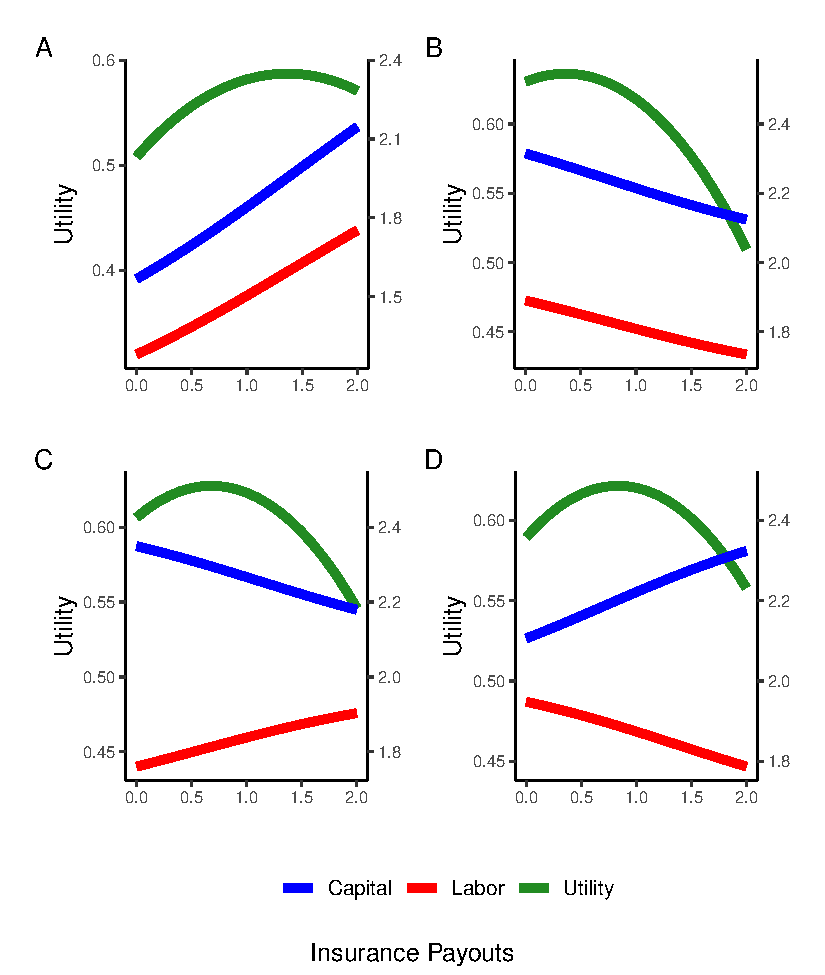
\includegraphics{ibi-behavior_files/figure-pdf/fig-ins-1.pdf}

}

\caption{\label{fig-ins}Fishers choose capital (blue line) and labor
(red line) to maximize utility (green line) for given insurance
contracts that offer more coverage along the x-axis. Fisher utility is
concave in all insurance payouts with CARA utility.}

\end{figure}

Figure~\ref{fig-ins} shows that conditions of
Proposition~\ref{prp-samre} can be satisfied, but it does not show the
conservation outcomes of index insurance. Fishers use the new choice of
inputs to change their overall harvest and thus impact on the biomass of
fish stocks. Harvest changes are influenced by the relative combination
of risk effects, mean production elastiticies, and the amount of
insurance (Figure~\ref{fig-multi-h-even}). Fishers reduce harvest more
aggressively with risk decreasing inputs when offered a set contract of
50\% coverage of pre-insurance profits (Panel A) relative to their
optimal insurance choice (Panel B). Allowing fishers to choose their
insurance coverage leads them to increase harvest more with risk
increasing inputs. A 50\% coverage is an overinvestment in insurance for
risk decreasing inputs and an underinvestment for risk increasing
inputs.

Mixed risk effects have more nuance in overall harvest as seen in the
top left and bottom right quadrants of each panel in
Figure~\ref{fig-multi-h-even}. Risk increasing inputs appear to dominant
risk reducing inputs leading to generally more increases in harvest. For
example, when an input has a risk increasing effect of 0.5, harvest
still increases even if the other input has a stronger risk reducing
effect at -0.7. The reduction in the risk decreasing output can outweigh
the increase in the risk increasing input if the risk decreasing effect
is much stronger than the risk increasing effect. For all risk effects
at -0.7, when the other input has a risk effect \textless0.3, harvest
decreases. In all cases, the change in harvest is quite small ranging
from 0.8\%-5\%.

\begin{figure}

{\centering 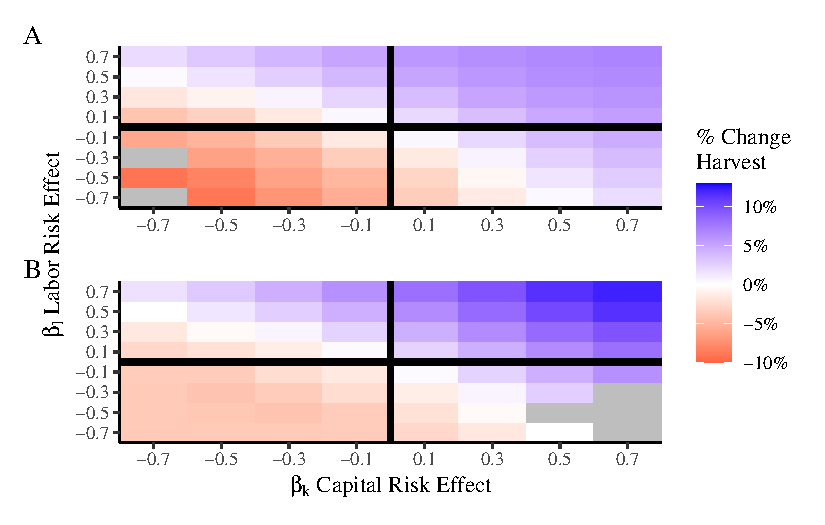
\includegraphics{ibi-behavior_files/figure-pdf/fig-multi-h-even-1.pdf}

}

\caption{\label{fig-multi-h-even}Percent change in fishing harvest when
fishers use index insurance with low mean elasticity values
(\(\alpha_{k,l}=0.25\)). In Panel A, Insurance payouts are a set
variable. In Panel B, fishers choose insurance payouts. Red colors show
overall decreases in harvest while blue colors show overall increases in
harvest. Grey boxes indicate simulations where it was not profitable to
fish at all with the given production inputs.}

\end{figure}

Increasing the mean elasticities exacerbates the discrepancies between
changes in harvest through index insurance
(Figure~\ref{fig-multi-h-even-hi}). When the productivity of harvest
(\(\alpha\)) is higher, the tradeoff between reducing variance and catch
changes. When the mean production elasticity is increased to 0.5, the
maximum amount of observed harvest is 45\% when fishers choose their
insurance levels while the greatest reduction is only 8\%. Higher mean
elasticities imply a greater change in harvest and profit with changes
in an input. Lowering use will have a proportionally greater tradeoff
between risk protection and income for risk decreasing inputs at higher
mean production elasticities.

\begin{figure}

{\centering 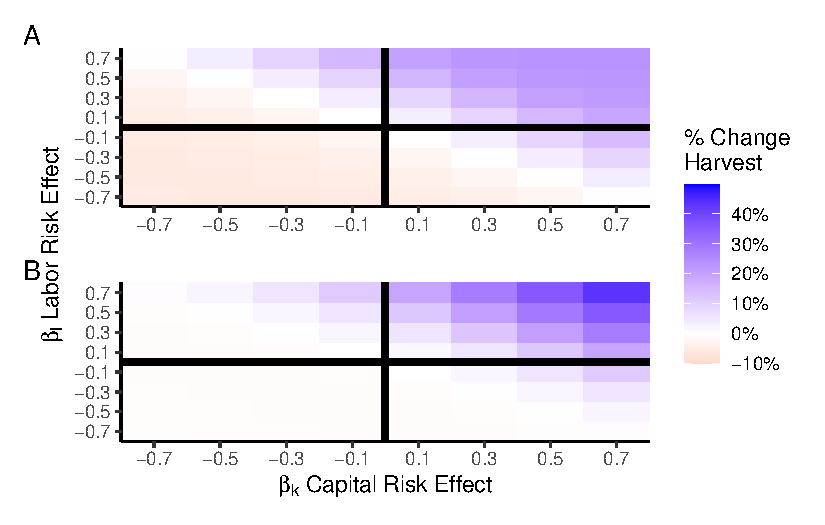
\includegraphics{ibi-behavior_files/figure-pdf/fig-multi-h-even-hi-1.pdf}

}

\caption{\label{fig-multi-h-even-hi}When fishers choose insurnace, they
drastically increase (blue) harvest with risk increasing relative to no
insurance harvest. Inputs share the same mean elasticity
(\(\alpha_{k,l}=0.5\)). Insurance payouts are exogenously set at 50\%
profits in Panel A. Insurance payouts are chosen in Panel B. Risk
aversion is set to 1. Weather variance is 0.5. Below the dotted line
show cases where harvest was reduced.}

\end{figure}

The magnitude of input use also changes based on the fisher risk
preferences, weather risk, and contract terms. We extract simulation
results where both inputs have the same risk effects and both have mean
production elasticities of 0.5 (\(\alpha_k=\alpha_l=0.5\)) to more
clearly isolate these effects (Figure~\ref{fig-multi-para}). More risk
averse fishers respond more aggressively to insurance and make
relatively more changes toward their input decisions (Panel A in
Figure~\ref{fig-multi-para}). Risk aversion implies more sensitivity
towards risk. The protection from insurance has greater marginal value
for more risk averse fishers. Greater marginal value of insurance means
they can invest less into risk reducing inputs than before, and have
more protection from greater shocks with risk increasing inputs.

Fisher input choice are much more responsive to insurance protection
from larger environmental risks (Panel B Figure~\ref{fig-multi-para}).
Similar to risk aversion, the greater the shocks the greater the
marginal value of insurance is to mitigate those shocks. In more
volatile environments, insurance provides significantly more income
smoothing leading to similar incentives as the higher risk aversion
example.

Trigger levels also influence fisher behavior in interesting ways. When
insurance covers more catastrophic events, such as shocks that are in
the 75th percentile, fishers respond more aggressively if they are using
risk decreasing inputs compared to risk increasing inputs (Panel C
Figure~\ref{fig-multi-para}). Payouts occur in disastrous events at
higher levels of coverage. When these larger shocks occur adding more
risk increasing inputs could lead to more catastrophic outcomes. The
incentive to increase input use is reduced in this case. Risk decreasing
inputs on the other hand are more easily substitutable with insurance
when greater shocks occur. Hence, the incentive for fishers to reduce
input use is greater.

\begin{figure}

{\centering 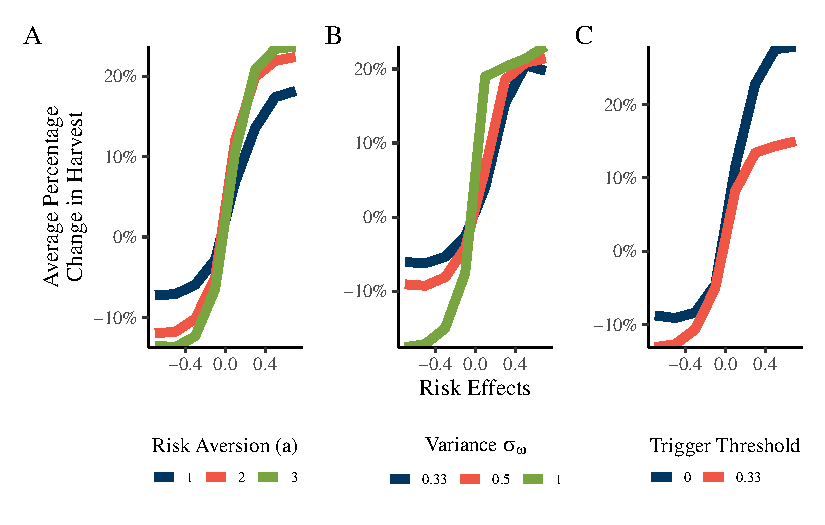
\includegraphics{ibi-behavior_files/figure-pdf/fig-multi-para-1.pdf}

}

\caption{\label{fig-multi-para}Risk Aversion (A), trigger level (B), and
weather variance (C) all influence the magnitude of change in harvest.
Mean production elasticity is 0.5 for both inputs. Average percent
change in harvest (y-axis) is summarized across all other parameter
combinations for each risk effect combination (x-axis) that are the same
for both inputs (e.g.~\(-0.4=\beta_k=\beta_l\))}

\end{figure}

\hypertarget{tbl-nor}{}
\begin{longtable}[t]{lllllr}
\caption{\label{tbl-nor}Percent change in input use and harvest for four Norwegian fisheries due
to index insurance induced moral hazards. }\tabularnewline

\toprule
 & Capital & Labor & Fuel & Harvest & \$\textbackslash{}gamma\$\\
\midrule
Coastal Seiners & 0\% & -2\% & 0\% & 0\% & 0.43\\
Coastal Groundfish & 20\% & 6\% & 8\% & 16\% & 1.24\\
Purse Seiners & -4\% & 0\% & -4\% & -6\% & 0.81\\
Groundfish Trawlers & -4\% & 0\% & 0\% & -2\% & 0.23\\
\bottomrule
\end{longtable}

\hypertarget{references}{%
\section*{References}\label{references}}
\addcontentsline{toc}{section}{References}

\hypertarget{refs}{}
\begin{CSLReferences}{1}{0}
\leavevmode\vadjust pre{\hypertarget{ref-Alvarez2006}{}}%
Alvarez, A., Schmidt, P., Alvarez, A. and Schmidt, P. (2006)
\href{https://doi.org/10.1007/s11123-006-0002-x}{Is skill more important
than luck in explaining fish catches?} \emph{J Prod Anal} \textbf{26},
15--25.

\leavevmode\vadjust pre{\hypertarget{ref-Asche2020}{}}%
Asche, F., Cojocaru, A.L., Pincinato, R.B.M. and Roll, K.H. (2020)
\href{https://doi.org/10.1007/s10640-019-00391-2}{Production risk in the
norwegian fisheries}. \emph{Environmental and Resource Economics}
\textbf{75}, 137--149.

\leavevmode\vadjust pre{\hypertarget{ref-Babcock1996}{}}%
Babcock, B.A. and Hennessy, D.A. (1996)
\href{https://doi.org/10.2307/1243713}{Input demand under yield and
revenue insurance}. \emph{American Journal of Agricultural Economics}
\textbf{78}, 416--427.

\leavevmode\vadjust pre{\hypertarget{ref-Barbeaux2020}{}}%
Barbeaux, S.J., Holsman, K. and Zador, S. (2020)
\href{https://doi.org/10.3389/fmars.2020.00703}{Marine heatwave stress
test of ecosystem-based fisheries management in the gulf of alaska
pacific cod fishery}. \emph{Frontiers in Marine Science} \textbf{7},
1--21.

\leavevmode\vadjust pre{\hypertarget{ref-Bulte2021}{}}%
Bulte, E. and Haagsma, R. (2021)
\href{https://doi.org/10.1007/s10640-021-00545-1}{The welfare effects of
index-based livestock insurance: Livestock herding on communal lands}.
\emph{Environmental and Resource Economics} \textbf{78}, 587--613.

\leavevmode\vadjust pre{\hypertarget{ref-Cai2016}{}}%
Cai, J. (2016) \href{https://doi.org/10.1257/pol.20130371}{The impact of
insurance provision on household production and financial decisions}.
\emph{American Economic Journal: Economic Policy} \textbf{8}, 44--88.

\leavevmode\vadjust pre{\hypertarget{ref-Carter2017}{}}%
Carter, M., Janvry, A.D., Sadoulet, E. and Sarris, A. (2017)
\href{https://doi.org/10.1146/annurev-resource-100516-053352}{Index
insurance for developing country agriculture: A reassessment}.
\emph{Annual Review of Resource Economics} \textbf{9}, 421--438.

\leavevmode\vadjust pre{\hypertarget{ref-Cavole2016}{}}%
Cavole, L.M., Demko, A.M., Diner, R.E., et al. (2016)
\href{https://doi.org/10.5670/oceanog.2016.32}{Biological impacts of the
2013--2015 warm-water anomaly in the northeast pacific: Winners, losers,
and the future}. \emph{Oceanography} \textbf{29}, 273--285.

\leavevmode\vadjust pre{\hypertarget{ref-Cheung2021}{}}%
Cheung, W.W.L., Frölicher, T.L., Lam, V.W.Y., et al. (2021)
\href{https://www.science.org}{Marine high temperature extremes amplify
the impacts of climate change on fish and fisheries}. \emph{Sci. Adv}
\textbf{7}.

\leavevmode\vadjust pre{\hypertarget{ref-Claassen2017}{}}%
Claassen, R., Langpap, C. and Wu, J. (2017)
\href{https://doi.org/10.1093/AJAE/AAW075}{Impacts of federal crop
insurance on land use and environmental quality}. \emph{American Journal
of Agricultural Economics} \textbf{99}, 592--613.

\leavevmode\vadjust pre{\hypertarget{ref-Clarke2016}{}}%
Clarke, D.J. (2016) \href{https://doi.org/10.1257/mic.20140103}{A theory
of rational demand for index insurance}. \emph{Journal: Microeconomics}
\textbf{8}, 283--306.

\leavevmode\vadjust pre{\hypertarget{ref-Collier2009}{}}%
Collier, B., Skees, J. and Barnett, B. (2009)
\href{https://doi.org/10.1057/gpp.2009.11}{Weather index insurance and
climate change: Opportunities and challenges in lower income countries}.
\emph{Geneva Papers on Risk and Insurance: Issues and Practice}
\textbf{34}, 401--424.

\leavevmode\vadjust pre{\hypertarget{ref-Deryugina2017}{}}%
Deryugina, T. and Konar, M. (2017)
\href{https://doi.org/10.1016/j.advwatres.2017.03.013}{Impacts of crop
insurance on water withdrawals for irrigation}. \emph{Advances in Water
Resources} \textbf{110}, 437--444.

\leavevmode\vadjust pre{\hypertarget{ref-Dougherty2021}{}}%
Dougherty, J.P., Gallenstein, R.A. and Mishra, K. (2021)
\href{https://doi.org/10.1093/jafeco/ejab003}{Impact of index insurance
on moral hazard in the agricultural credit market: Theory and evidence
from ghana}. \emph{Journal of African Economies} \textbf{00}, 1--31.

\leavevmode\vadjust pre{\hypertarget{ref-Eggert2004}{}}%
Eggert, H. and Tveteras, R. (2004) Stochastic production and
heterogeneous risk preferences: Commercial fishers' gear choices.
\emph{American Journal of Agricultural Economics} \textbf{86}, 199--212.

\leavevmode\vadjust pre{\hypertarget{ref-Elabed2016}{}}%
Elabed, G. and Carter, M. (2018) Ex-ante impacts of agricultural
insurance: Evidence from a field experiment in mali.

\leavevmode\vadjust pre{\hypertarget{ref-fao2020}{}}%
FAO (2020) \href{https://doi.org/10.4060/ca9229en}{The state of world
fisheries and aquaculture 2020. Sustinability in action}. \emph{INFORM}
\textbf{32}.

\leavevmode\vadjust pre{\hypertarget{ref-fao2022}{}}%
FAO (2022) World review of capture fisheries and aquaculture insurance
2022.

\leavevmode\vadjust pre{\hypertarget{ref-Fisher2019}{}}%
Fisher, E., Hellin, J., Greatrex, H. and Jensen, N. (2019)
\href{https://doi.org/10.1111/dpr.12387}{Index insurance and climate
risk management: Addressing social equity}. \emph{Development Policy
Review} \textbf{37}, 581--602.

\leavevmode\vadjust pre{\hypertarget{ref-Goodwin2004}{}}%
Goodwin, B.K., Vandeveer, M.L. and Deal, J.L. (2004) An empirical
analysis of acreage effects of participation in the federal crop
insurance program. \emph{American Journal of Agricultural Economics}
\textbf{86}, 1058--1077.

\leavevmode\vadjust pre{\hypertarget{ref-Heck2021}{}}%
Heck, N., Beck, M.W. and Reguero, B. (2021)
\href{https://doi.org/10.1016/j.marpol.2021.104698}{Storm risk and
marine fisheries: A global assessment}. \emph{Marine Policy}
\textbf{132}, 104698.

\leavevmode\vadjust pre{\hypertarget{ref-Holland2008}{}}%
Holland, D.S. (2008)
\href{https://doi.org/10.1086/mre.23.3.42629621}{Are fishermen rational?
A fishing expedition}. \emph{Marine Resource Economics} \textbf{23},
325--344.

\leavevmode\vadjust pre{\hypertarget{ref-horowitz1993}{}}%
Horowitz, J. and Lichtenberg, E. (1993) Insurance, moral hazard, and
chemical use in agriculture. \emph{American Journal of Agricultral
Economics} \textbf{75}, 926--935.

\leavevmode\vadjust pre{\hypertarget{ref-Jardine2020}{}}%
Jardine, S.L., Fisher, M.C., Moore, S.K. and Samhouri, J.F. (2020)
\href{https://doi.org/10.1016/j.ecolecon.2020.106691}{Inequality in the
economic impacts from climate shocks in fisheries: The case of harmful
algal blooms}. \emph{Ecological Economics} \textbf{176}.

\leavevmode\vadjust pre{\hypertarget{ref-Just1979}{}}%
Just, R.E. and Pope, R.D. (1979) Production function estimation and
related risk considerations. \emph{Source: American Journal of
Agricultural Economics} \textbf{61}, 276--284.

\leavevmode\vadjust pre{\hypertarget{ref-Just1978}{}}%
Just, R.E. and Pope, R.D. (1978)
\href{https://doi.org/10.1016/0304-4076(78)90006-4}{Stochastic
specification of production functions and economic implications}.
\emph{Journal of Econometrics} \textbf{7}, 67--86.

\leavevmode\vadjust pre{\hypertarget{ref-Kasperski2013}{}}%
Kasperski, S. and Holland, D.S. (2013)
\href{https://doi.org/10.1073/pnas.1212278110}{Income diversification
and risk for fishermen}. \emph{Proceedings of the National Academy of
Sciences of the United States of America} \textbf{110}, 2076--2081.

\leavevmode\vadjust pre{\hypertarget{ref-Kirkley1998}{}}%
Kirkley, J. and Strand, I.E. (1998) Characterizing managerial skill and
technical efficiency in a fishery. \emph{Journal of Productivity
Analysis} \textbf{9}, 145--160.

\leavevmode\vadjust pre{\hypertarget{ref-Kompas2004}{}}%
Kompas, T., Che, T.N. and Grafton, R.Q. (2004)
\href{https://doi.org/10.1080/0003684042000218561}{Technical efficiency
effects of input controls: Evidence from australia's banana prawn
fishery}. \emph{Applied Economics} \textbf{36}, 1631--1641.

\leavevmode\vadjust pre{\hypertarget{ref-Lichtenberg2022}{}}%
Lichtenberg, E. and Iglesias, E. (2022)
\href{https://doi.org/10.1016/j.jdeveco.2022.102883}{Index insurance and
basis risk: A reconsideration}. \emph{Journal of Development Economics}
\textbf{158}.

\leavevmode\vadjust pre{\hypertarget{ref-Mahul2001}{}}%
Mahul, O. (2001) \href{https://doi.org/10.1111/0002-9092.00180}{Optimal
insurance against climatic experience}. \emph{American Journal of
Agricultural Economics} \textbf{83}, 593--604.

\leavevmode\vadjust pre{\hypertarget{ref-Maltby2023}{}}%
Maltby, K.M., Acosta, L., Townhill, B., Touza, J., White, P. and Mangi,
S.C. (2023) \href{https://doi.org/10.1093/icesjms/fsac003}{Exploring
fishers' perceptions of index insurance and coral reef health in the
context of climate-driven changes in extreme events}. \emph{ICES Journal
of Marine Science} \textbf{80}, 2210--2221.

\leavevmode\vadjust pre{\hypertarget{ref-Merino2022}{}}%
Merino, G., Urtizberea, A., Fu, D., et al. (2022)
\href{https://doi.org/10.1016/j.fishres.2022.106478}{Investigating
trends in process error as a diagnostic for integrated fisheries stock
assessments}. \emph{Fisheries Research} \textbf{256}.

\leavevmode\vadjust pre{\hypertarget{ref-gibbons1993}{}}%
Mesterton-Gibbons, M. (1993)
\href{https://doi.org/10.1111/j.1939-7445.1993.tb00143.x}{Game-theoretic
resource modeling}. \emph{Natural Resource Modeling} \textbf{7},
93--147.

\leavevmode\vadjust pre{\hypertarget{ref-Mishra2005}{}}%
Mishra, A.K., Nimon, R.W. and El-Osta, H.S. (2005)
\href{https://doi.org/10.1016/j.jenvman.2004.08.003}{Is moral hazard
good for the environment? Revenue insurance and chemical input use}.
\emph{Journal of Environmental Management} \textbf{74}, 11--20.

\leavevmode\vadjust pre{\hypertarget{ref-muller2011}{}}%
Müller, B., Quaas, M.F., Frank, K. and Baumgärtner, S. (2011)
\href{https://doi.org/10.1016/j.ecolecon.2011.06.011}{Pitfalls and
potential of institutional change: Rain-index insurance and the
sustainability of rangeland management}. \emph{Ecological Economics}
\textbf{70}, 2137--2144.

\leavevmode\vadjust pre{\hypertarget{ref-Murkowski2022}{}}%
Murkowski, L. (2022) Working waterfronts framework: A plan to grow and
support alaska's coastal and river communities.

\leavevmode\vadjust pre{\hypertarget{ref-Oken2021}{}}%
Oken, K.L., Holland, D.S. and Punt, A.E. (2021)
\href{https://doi.org/10.1002/eap.2307}{The effects of population
synchrony, life history, and access constraints on benefits from fishing
portfolios}. \emph{Ecological Applications} \textbf{0}, 1--16.

\leavevmode\vadjust pre{\hypertarget{ref-Outreville2014}{}}%
Outreville, J.F. (2014) Risk aversion, risk behavior, and demand for
insurance: A survey. \emph{Source: Journal of Insurance Issues}
\textbf{37}, 158--186.

\leavevmode\vadjust pre{\hypertarget{ref-Pandori2019}{}}%
Pandori, L.L.M. and Sorte, C.J.B. (2019)
\href{https://doi.org/10.1111/oik.05886}{The weakest link: Sensitivity
to climate extremes across life stages of marine invertebrates}.
\emph{Oikos} \textbf{128}, 621--629.

\leavevmode\vadjust pre{\hypertarget{ref-Pfeiffer2020}{}}%
Pfeiffer, L. (2020) \href{https://doi.org/10.1093/icesjms/fsaa145}{How
storms affect fishers' decisions about going to sea}. \emph{ICES Journal
of Marine Science} \textbf{77}, 2753--2762.

\leavevmode\vadjust pre{\hypertarget{ref-Pfeiffer2022}{}}%
Pfeiffer, L., Petesch, T. and Vasan, T. (2022)
\href{https://doi.org/10.1086/716856}{A safer catch? The role of
fisheries management in fishing safety}. \emph{Marine Resource
Economics} \textbf{37}, 1--33.

\leavevmode\vadjust pre{\hypertarget{ref-Quaas2008}{}}%
Quaas, M.F. and Baumgärtner, S. (2008)
\href{https://doi.org/10.1016/j.ecolecon.2007.07.004}{Natural vs.
Financial insurance in the management of public-good ecosystems}.
\emph{Ecological Economics} \textbf{65}, 397--406.

\leavevmode\vadjust pre{\hypertarget{ref-Ramaswami1993}{}}%
Ramaswami, B. (1993) Supply response to agricultural insurance: Risk
reduction and moral hazard effects. \emph{American Journal of
Agricultural Economics} \textbf{75}, 914--925.

\leavevmode\vadjust pre{\hypertarget{ref-Reimer2017}{}}%
Reimer, M.N., Abbott, J.K. and Wilen, J.E. (2017)
\href{https://doi.org/10.1086/690678}{Fisheries production: Management
institutions, spatial choice, and the quest for policy invariance}.
\emph{Marine Resource Economics} \textbf{32}, 143--168.

\leavevmode\vadjust pre{\hypertarget{ref-rogers2019}{}}%
Rogers, L.A., Griffin, R., Young, T., Fuller, E., Martin, K.S. and
Pinsky, M.L. (2019)
\href{https://doi.org/10.1038/s41558-019-0503-z}{Shifting habitats
expose fishing communities to risk under climate change}. \emph{Nature
Climate Change} \textbf{9}, 512--516.

\leavevmode\vadjust pre{\hypertarget{ref-Sainsbury2019}{}}%
Sainsbury, N.C., Turner, R.A., Townhill, B.L., Mangi, S.C. and Pinnegar,
J.K. (2019) \href{https://doi.org/10.1038/s41558-019-0645-z}{The
challenges of extending climate risk insurance to fisheries}.
\emph{Nature Climate Change} \textbf{9}, 896--897.

\leavevmode\vadjust pre{\hypertarget{ref-Sethi2010}{}}%
Sethi, S.A. (2010)
\href{https://doi.org/10.1111/j.1467-2979.2010.00363.x}{Risk management
for fisheries}. \emph{Fish and Fisheries} \textbf{11}, 341--365.

\leavevmode\vadjust pre{\hypertarget{ref-Sibiko2020}{}}%
Sibiko, K.W. and Qaim, M. (2020)
\href{https://doi.org/10.1007/s12571-019-00987-y}{Weather index
insurance, agricultural input use, and crop productivity in kenya}.
\emph{Food Security} \textbf{12}, 151--167.

\leavevmode\vadjust pre{\hypertarget{ref-Sims2018}{}}%
Sims, C., Horan, R.D. and Meadows, B. (2018)
\href{https://doi.org/10.1111/NRM.12191}{Come on feel the noise:
Ecological foundations in stochastic bioeconomic models}. \emph{Natural
Resource Modeling} \textbf{31}.

\leavevmode\vadjust pre{\hypertarget{ref-Smith2023}{}}%
Smith, K.E., Burrows, M.T., Hobday, A.J., et al. (2023)
\href{https://doi.org/10.1146/annurev-marine-032122-121437}{Biological
impacts of marine heatwaves}. \emph{Annual Review of Marine Science}
\textbf{15}, 1--27.

\leavevmode\vadjust pre{\hypertarget{ref-Smith2005}{}}%
Smith, M.D. and Wilen, J.E. (2005) Heterogeneous and correlated risk
preferences in commercial fishermen: The perfect storm dilemma.
\emph{The Journal of Risk and Uncertainty} \textbf{31}, 1--53.

\leavevmode\vadjust pre{\hypertarget{ref-Smith1996}{}}%
Smith, V.H. and Goodwin, B.K. (1996)
\href{https://doi.org/10.2307/1243714}{Crop insurance, moral hazard, and
agricultural chemical use}. \emph{The Economics of Agri-Environmental
Policy} \textbf{2}, 169--179.

\leavevmode\vadjust pre{\hypertarget{ref-stoeffler2022}{}}%
Stoeffler, Q., Carter, M., Guirkinger, C. and Gelade, W. (2022)
\href{https://doi.org/10.1093/wber}{The spillover impact of index
insurance on agricultural investment by cotton farmers in burkina faso}.
\emph{The World Bank Economic Review} \textbf{36}, 114--140.

\leavevmode\vadjust pre{\hypertarget{ref-Sumaila2012}{}}%
Sumaila, U.R., Cheung, W., Dyck, A., et al. (2012)
\href{https://doi.org/10.1371/journal.pone.0040542}{Benefits of
rebuilding global marine fisheries outweigh costs}. \emph{PLoS ONE}
\textbf{7}.

\leavevmode\vadjust pre{\hypertarget{ref-sumalia2020}{}}%
Sumaila, U.R., Walsh, M., Hoareau, K., et al. (2020)
\href{https://www.oceanpanel.org/blue-}{Ocean finance: Financing the
transition to a sustainable ocean economy}.

\leavevmode\vadjust pre{\hypertarget{ref-Teh2013}{}}%
Teh, L.C.L. and Sumaila, U.R. (2013)
\href{https://doi.org/10.1111/j.1467-2979.2011.00450.x}{Contribution of
marine fisheries to worldwide employment}. \emph{Fish and Fisheries}
\textbf{14}, 77--88.

\leavevmode\vadjust pre{\hypertarget{ref-Tilman2018}{}}%
Tilman, A.R., Levin, S. and Watson, J.R. (2018)
\href{https://doi.org/10.1016/j.jtbi.2018.06.003}{Revenue-sharing clubs
provide economic insurance and incentives for sustainability in
common-pool resource systems keywords: Risk insurance social-ecological
systems fisheries management sustainability complex adaptive systems
agent-based model common-poo}. \emph{Journal of Theoretical Biology}
\textbf{454}, 205--214.

\leavevmode\vadjust pre{\hypertarget{ref-Tromeur2021}{}}%
Tromeur, E., Doyen, L., Tarizzo, V., Little, L.R., Jennings, S. and
Thébaud, O. (2021)
\href{https://doi.org/10.1016/j.ecolecon.2021.107178}{Risk averse
policies foster bio-economic sustainability in mixed fisheries}.
\emph{Ecological Economics} \textbf{190}.

\leavevmode\vadjust pre{\hypertarget{ref-Wabnitz2019}{}}%
Wabnitz, C.C.C. and Blasiak, R. (2019)
\href{https://doi.org/10.1016/j.marpol.2019.103526}{The rapidly changing
world of ocean finance}. \emph{Marine Policy} \textbf{107}, 103526.

\leavevmode\vadjust pre{\hypertarget{ref-Watson2023}{}}%
Watson, J.R., Spillman, C.M., Little, L.R., Hobday, A.J. and Levin, P.S.
(2023) \href{https://doi.org/10.1093/icesjms/fsad175}{Enhancing the
resilience of blue foods to climate shocks using insurance}. \emph{ICES
Journal of Marine Science} \textbf{80}, 2457--2469.

\leavevmode\vadjust pre{\hypertarget{ref-White2012}{}}%
White, T.K. and Hoppe, R.A. (2012)
\href{https://www.ers.usda.gov}{Changing farm structure and the
distribution of farm payments and federal crop insurance}.

\leavevmode\vadjust pre{\hypertarget{ref-Wu2020}{}}%
Wu, S., Goodwin, B.K. and Coble, K. (2020)
\href{https://doi.org/10.1111/agec.12545}{Moral hazard and subsidized
crop insurance}. \emph{Agricultural Economics (United Kingdom)}
\textbf{51}, 131--142.

\end{CSLReferences}



\end{document}
